\begin{itemize}
\tightlist
\item
  \protect\hyperlink{11-lake}{11 Lake}

  \begin{itemize}
  \tightlist
  \item
    \protect\hyperlink{111-lake-surface-conditions-lakebc-100-written-in-jan-2021}{11.1
    Lake surface conditions \texttt{{[}LAKEBC{]}} {[}100\% Written in
    Jan, 2021{]}}

    \begin{itemize}
    \tightlist
    \item
      \protect\hyperlink{1111-lake-surface-albedo-lakealb}{11.1.1. lake
      surface albedo \texttt{{[}LAKEALB{]}}}
    \item
      \protect\hyperlink{1112-lake-surface-roughness-lakez0f}{11.1.2
      Lake surface roughness \texttt{{[}LAKEZ0F{]}}}
    \end{itemize}
  \item
    \protect\hyperlink{112-lake-surface-heat-balance-lakehb-100-written-in-jan-2021}{11.2
    Lake surface heat balance \texttt{{[}LAKEHB{]}} {[}100\% Written in
    Jan, 2021{]}}
  \item
    \protect\hyperlink{113-lake-ice-submodel-lakeic-100-written-in-jan-2021}{11.3
    Lake ice submodel \texttt{{[}LAKEIC{]}} {[}100\% Written in Jan,
    2021{]}}

    \begin{itemize}
    \tightlist
    \item
      \protect\hyperlink{1131-heat-flux-and-growth-rate-modulefiheatl}{11.3.1
      Heat Flux and Growth Rate \texttt{MODULE{[}FIHEATL{]}}}
    \item
      \protect\hyperlink{1132-sublimation-of-sea-icemodulefwaterl}{11.3.2
      Sublimation of Sea Ice\texttt{MODULE{[}FWATERL{]}}}
    \item
      \protect\hyperlink{1133-update-snow-and-ice-volume-pcmpctl}{11.3.3
      Update snow and ice volume \texttt{{[}PCMPCTL{]}}}
    \item
      \protect\hyperlink{1134-growth-and-melting-pthickl}{11.3.4 Growth
      and Melting \texttt{{[}PTHICKL{]}}}
    \end{itemize}
  \item
    \protect\hyperlink{114-physical-formulation-processes-lakepo-20-written-in-jan-2021}{11.4
    Physical formulation \& processes \texttt{{[}LAKEPO{]}} {[}20\%
    Written in Jan, 2021{]}}

    \begin{itemize}
    \tightlist
    \item
      \protect\hyperlink{set-parameters}{Set parameters}

      \begin{itemize}
      \tightlist
      \item
        \protect\hyperlink{diffusion-tracer-flux-vdiffl}{Diffusion
        tracer flux \texttt{{[}VDIFFL{]}}}
      \item
        \protect\hyperlink{1132-estimate-the-advection-and-diffusion-terms-of-the-tracer-equations-flxtrcl}{11.3.2
        Estimate the advection and diffusion terms of the tracer
        equations \texttt{{[}FLXTRCL{]}}}
      \item
        \protect\hyperlink{slvtrcl}{SLVTRCL}
      \item
        \protect\hyperlink{ovturnl}{OVTURNL}
      \end{itemize}
    \item
      \protect\hyperlink{1131-setting-vertical-diffusion-and-viscosity-coefficients-vdiffl}{11.3.1
      Setting vertical diffusion and viscosity coefficients
      \texttt{{[}VDIFFL{]}}}
    \item
      \protect\hyperlink{thomasl}{THOMASL}
    \item
      \protect\hyperlink{1134-convective-adjustment-for-the-unstable-water-column-ovtsetl}{11.3.4
      Convective adjustment for the unstable water column
      \texttt{{[}OVTSETL{]}}}
    \end{itemize}
  \end{itemize}
\end{itemize}

\hypertarget{lake}{%
\section{11 Lake}\label{lake}}

Up to and including the calculation of the surface flux (11.1-11.2), the
method is derived from the land surface model MATSIRO, while the
calculation below the lake ice (11.3-11.4) is derived from the ocean
model COCO. (The description in this section is also based on Emori
(2000) for the first half and
\href{https://ccsr.aori.u-tokyo.ac.jp/~hasumi/COCO/coco4.pdf}{Hasumi
(2015)} for the second half.) For practical use, note, for example, that
the unit of temperature is \(\mathrm{K}\) until section 11.2, while it
is \(\mathrm{°C}\) after section 11.3. It is also noted that because the
second half part is based on the old version of COCO, hence it is
slightly different from the MIROC6-AOGCM and
\href{https://ccsr.aori.u-tokyo.ac.jp/~hasumi/COCO/coco4.pdf}{Hasumi
(2015)}.

Dimensions of the lake scheme is defined in \texttt{include/zkg21c.F}.
\texttt{KLMAX} is the number of vertical layers set to 5 in
MIROC6/MATSIRO6. \texttt{NLTDIM} is the number of tracers, 1:temperature
2:salt. Since the vertical layers are actually from \texttt{KLSTR=2} to
\texttt{KLEND=KLMAX+1}, \texttt{NLZDIM\ =\ KLMAX+KLSTR} exists as a
parameter for management.

Maximum and minimum thresholds for the lake scheme are given in
\texttt{matdrv.F}.

\setlength\LTleft{0pt}\setlength\LTright{0pt}\begin{longtable}[]{@{}lllll@{}}
\toprule\relax
\begin{minipage}[b]{0.30\columnwidth}\raggedright
Meaning\strut
\end{minipage} & \begin{minipage}[b]{0.15\columnwidth}\raggedright
Presentation\strut
\end{minipage} & \begin{minipage}[b]{0.09\columnwidth}\raggedright
Variable\strut
\end{minipage} & \begin{minipage}[b]{0.14\columnwidth}\raggedright
unit\strut
\end{minipage} & \begin{minipage}[b]{0.18\columnwidth}\raggedright
value\strut
\end{minipage}\tabularnewline
\midrule\relax
\endhead
\begin{minipage}[t]{0.30\columnwidth}\raggedright
minimum depth of lake\strut
\end{minipage} & \begin{minipage}[t]{0.15\columnwidth}\raggedright
\(h_{min}\)\strut
\end{minipage} & \begin{minipage}[t]{0.09\columnwidth}\raggedright
HHMIN\strut
\end{minipage} & \begin{minipage}[t]{0.14\columnwidth}\raggedright
\(\mathrm{cm}\)\strut
\end{minipage} & \begin{minipage}[t]{0.18\columnwidth}\raggedright
\(10^\times 10^{2}\)\strut
\end{minipage}\tabularnewline
\begin{minipage}[t]{0.30\columnwidth}\raggedright
maximum of surface high anomaly\strut
\end{minipage} & \begin{minipage}[t]{0.15\columnwidth}\raggedright
\(\eta_{max}\)\strut
\end{minipage} & \begin{minipage}[t]{0.09\columnwidth}\raggedright
HAMAX\strut
\end{minipage} & \begin{minipage}[t]{0.14\columnwidth}\raggedright
\(\mathrm{cm}\)\strut
\end{minipage} & \begin{minipage}[t]{0.18\columnwidth}\raggedright
\(10^\times 10^{2}\)\strut
\end{minipage}\tabularnewline
\begin{minipage}[t]{0.30\columnwidth}\raggedright
maximum of lake snow\strut
\end{minipage} & \begin{minipage}[t]{0.15\columnwidth}\raggedright
\(h_{snow,max}\)\strut
\end{minipage} & \begin{minipage}[t]{0.09\columnwidth}\raggedright
HSMAX\strut
\end{minipage} & \begin{minipage}[t]{0.14\columnwidth}\raggedright
\(\mathrm{cm}\)\strut
\end{minipage} & \begin{minipage}[t]{0.18\columnwidth}\raggedright
\(10^\times 10^{2}\)\strut
\end{minipage}\tabularnewline
\begin{minipage}[t]{0.30\columnwidth}\raggedright
maximum of lake ice thickness\strut
\end{minipage} & \begin{minipage}[t]{0.15\columnwidth}\raggedright
\(h_{ice,max}\)\strut
\end{minipage} & \begin{minipage}[t]{0.09\columnwidth}\raggedright
HIMAX\strut
\end{minipage} & \begin{minipage}[t]{0.14\columnwidth}\raggedright
\(\mathrm{cm}\)\strut
\end{minipage} & \begin{minipage}[t]{0.18\columnwidth}\raggedright
\(10^\times 10^{2}\)\strut
\end{minipage}\tabularnewline
\bottomrule
\end{longtable}

\hypertarget{lake-surface-conditions-lakebc-100-written-in-jan-2021}{%
\subsection{\texorpdfstring{11.1 Lake surface conditions
\texttt{{[}LAKEBC{]}} {[}100\% Written in Jan,
2021{]}}{11.1 Lake surface conditions {[}LAKEBC{]} {[}100\% Written in Jan, 2021{]}}}\label{lake-surface-conditions-lakebc-100-written-in-jan-2021}}

\begin{itemize}
\tightlist
\item
  Outputs
\end{itemize}

\setlength\LTleft{0pt}\setlength\LTright{0pt}\begin{longtable}[]{@{}lllll@{}}
\toprule\relax
Meaning & Presentation & Variable & dimension & unit\tabularnewline
\midrule\relax
\endhead
surface albedo & \(\alpha\) & GRALB & IJLSDM, NRDIR, NRBND &
-\tabularnewline
surface roughness & \(r_0\) & GRZ0 & IJLSDM, NTYZ0 &\tabularnewline
heat flux & \(G\) & FOGFLX & IJLSDM &\tabularnewline
heat diffusion coefficient & \(\frac{\partial G}{\partial T}\) & DGFDS &
IJLSDM &\tabularnewline
\bottomrule
\end{longtable}

\begin{itemize}
\tightlist
\item
  Inputs
\end{itemize}

\setlength\LTleft{0pt}\setlength\LTright{0pt}\begin{longtable}[]{@{}lllll@{}}
\toprule\relax
Meaning & Presentation & Variable & dimension & unit\tabularnewline
\midrule\relax
\endhead
skin temperature & \(T_s\) & GRTS & IJLSDM &
\(\mathrm{K}\)\tabularnewline
ice base temperature & \(T_b\) & GRTB & IJLSDM &\tabularnewline
lake ice amount & \(Ic\) & GRICE & IJLSDM &\tabularnewline
snow amount & \(Sn\) & GRSNW & IJLSDM &\tabularnewline
lake ice concentration & \(R_{ice}\) & GRICR & IJLSDM &\tabularnewline
u surface wind & \(U_0\) & GDUA & IJLSDM &\tabularnewline
v surface wind & \(V_0\) & GDVA & IJLSDM &\tabularnewline
cos(solar zenith) & \(\mathrm{cos}(\theta)\) & RCOSZ & IJLSDM
&\tabularnewline
\bottomrule
\end{longtable}

\begin{itemize}
\tightlist
\item
  Internal work variables
\end{itemize}

\setlength\LTleft{0pt}\setlength\LTright{0pt}\begin{longtable}[]{@{}lllll@{}}
\toprule\relax
Meaning & Presentation & Variable & dimension & unit\tabularnewline
\midrule\relax
\endhead
snow fraction & \(R_{snow}\) & GRSNR & IJLSDM & -\tabularnewline
& \(T_m^{max}-T_m^{min}\) & TALSNX & IJLSDM &\tabularnewline
& \(\alpha_{snow(2,b)}-\alpha_{snow(1,b)}\) & ALBSNX & IJLSDM
&\tabularnewline
& \(\alpha_0\) & ALB0 & IJLSDM &\tabularnewline
& tmp & DALB & IJLSDM &\tabularnewline
& \(F(T_s)\) & TFACT & IJLSDM &\tabularnewline
& \(\alpha''\) & ALBX & IJLSDM &\tabularnewline
& \(r'\) & Z00 & IJLSDM &\tabularnewline
& & DZ0 & IJLSDM &\tabularnewline
heat diffusion coefficient & & DFGT & IJLSDM &\tabularnewline
& & DFGX & IJLSDM &\tabularnewline
\bottomrule
\end{longtable}

\begin{itemize}
\tightlist
\item
  Internal parameters
\end{itemize}

\setlength\LTleft{0pt}\setlength\LTright{0pt}\begin{longtable}[]{@{}lllll@{}}
\toprule\relax
\begin{minipage}[b]{0.19\columnwidth}\raggedright
Meaning\strut
\end{minipage} & \begin{minipage}[b]{0.15\columnwidth}\raggedright
Presentation\strut
\end{minipage} & \begin{minipage}[b]{0.11\columnwidth}\raggedright
Variable\strut
\end{minipage} & \begin{minipage}[b]{0.04\columnwidth}\raggedright
unit\strut
\end{minipage} & \begin{minipage}[b]{0.37\columnwidth}\raggedright
Header\strut
\end{minipage}\tabularnewline
\midrule\relax
\endhead
\begin{minipage}[t]{0.19\columnwidth}\raggedright
diffusion coef. of snow\strut
\end{minipage} & \begin{minipage}[t]{0.15\columnwidth}\raggedright
\(D_{snow}\)\strut
\end{minipage} & \begin{minipage}[t]{0.11\columnwidth}\raggedright
DFSNOW\strut
\end{minipage} & \begin{minipage}[t]{0.04\columnwidth}\raggedright
\strut
\end{minipage} & \begin{minipage}[t]{0.37\columnwidth}\raggedright
\(0.4\)\strut
\end{minipage}\tabularnewline
\begin{minipage}[t]{0.19\columnwidth}\raggedright
maximum snow depth\strut
\end{minipage} & \begin{minipage}[t]{0.15\columnwidth}\raggedright
\strut
\end{minipage} & \begin{minipage}[t]{0.11\columnwidth}\raggedright
SNWDMX\strut
\end{minipage} & \begin{minipage}[t]{0.04\columnwidth}\raggedright
\strut
\end{minipage} & \begin{minipage}[t]{0.37\columnwidth}\raggedright
\(5.0\)\strut
\end{minipage}\tabularnewline
\begin{minipage}[t]{0.19\columnwidth}\raggedright
minimum snow\strut
\end{minipage} & \begin{minipage}[t]{0.15\columnwidth}\raggedright
\strut
\end{minipage} & \begin{minipage}[t]{0.11\columnwidth}\raggedright
EPSSNW\strut
\end{minipage} & \begin{minipage}[t]{0.04\columnwidth}\raggedright
\strut
\end{minipage} & \begin{minipage}[t]{0.37\columnwidth}\raggedright
\(1.0\times 10^{-8}\)\strut
\end{minipage}\tabularnewline
\begin{minipage}[t]{0.19\columnwidth}\raggedright
ice forming snow\strut
\end{minipage} & \begin{minipage}[t]{0.15\columnwidth}\raggedright
\strut
\end{minipage} & \begin{minipage}[t]{0.11\columnwidth}\raggedright
SNWMAX\strut
\end{minipage} & \begin{minipage}[t]{0.04\columnwidth}\raggedright
\strut
\end{minipage} & \begin{minipage}[t]{0.37\columnwidth}\raggedright
\(1000.0\)\strut
\end{minipage}\tabularnewline
\begin{minipage}[t]{0.19\columnwidth}\raggedright
snow albedo\strut
\end{minipage} & \begin{minipage}[t]{0.15\columnwidth}\raggedright
\(\alpha_{snow(d,b)}\)\strut
\end{minipage} & \begin{minipage}[t]{0.11\columnwidth}\raggedright
ABLSNW(2, NRBND)\strut
\end{minipage} & \begin{minipage}[t]{0.04\columnwidth}\raggedright
\strut
\end{minipage} & \begin{minipage}[t]{0.37\columnwidth}\raggedright
\(0.75, 0.5, 0.75, 0.5, 0.0, 0.0\)\strut
\end{minipage}\tabularnewline
\begin{minipage}[t]{0.19\columnwidth}\raggedright
temperature for albedo change\strut
\end{minipage} & \begin{minipage}[t]{0.15\columnwidth}\raggedright
\(T_m^{min}, T_m^{max}\)\strut
\end{minipage} & \begin{minipage}[t]{0.11\columnwidth}\raggedright
TALSNW(2)\strut
\end{minipage} & \begin{minipage}[t]{0.04\columnwidth}\raggedright
\strut
\end{minipage} & \begin{minipage}[t]{0.37\columnwidth}\raggedright
\(258.15, 273.15\)\strut
\end{minipage}\tabularnewline
\begin{minipage}[t]{0.19\columnwidth}\raggedright
roughness of snow\strut
\end{minipage} & \begin{minipage}[t]{0.15\columnwidth}\raggedright
\(r_{snow}\)\strut
\end{minipage} & \begin{minipage}[t]{0.11\columnwidth}\raggedright
Z0SNW(NTYZ0)\strut
\end{minipage} & \begin{minipage}[t]{0.04\columnwidth}\raggedright
\strut
\end{minipage} & \begin{minipage}[t]{0.37\columnwidth}\raggedright
\(1.0\times 10^{-2}, 1.0\times 10^{-3}, 1.0\times 10^{-3}\)\strut
\end{minipage}\tabularnewline
\begin{minipage}[t]{0.19\columnwidth}\raggedright
snow amount for fraction=1\strut
\end{minipage} & \begin{minipage}[t]{0.15\columnwidth}\raggedright
\strut
\end{minipage} & \begin{minipage}[t]{0.11\columnwidth}\raggedright
SNWCRT\strut
\end{minipage} & \begin{minipage}[t]{0.04\columnwidth}\raggedright
\strut
\end{minipage} & \begin{minipage}[t]{0.37\columnwidth}\raggedright
\(100.0\)\strut
\end{minipage}\tabularnewline
\begin{minipage}[t]{0.19\columnwidth}\raggedright
snow density\strut
\end{minipage} & \begin{minipage}[t]{0.15\columnwidth}\raggedright
\strut
\end{minipage} & \begin{minipage}[t]{0.11\columnwidth}\raggedright
SNWDEN\strut
\end{minipage} & \begin{minipage}[t]{0.04\columnwidth}\raggedright
\strut
\end{minipage} & \begin{minipage}[t]{0.37\columnwidth}\raggedright
\(400.0\)\strut
\end{minipage}\tabularnewline
\begin{minipage}[t]{0.19\columnwidth}\raggedright
diffusion coef. of lake ice\strut
\end{minipage} & \begin{minipage}[t]{0.15\columnwidth}\raggedright
\(D_{ice}\)\strut
\end{minipage} & \begin{minipage}[t]{0.11\columnwidth}\raggedright
DFICE\strut
\end{minipage} & \begin{minipage}[t]{0.04\columnwidth}\raggedright
\strut
\end{minipage} & \begin{minipage}[t]{0.37\columnwidth}\raggedright
\(2.00\)\strut
\end{minipage}\tabularnewline
\begin{minipage}[t]{0.19\columnwidth}\raggedright
lake ice albedo\strut
\end{minipage} & \begin{minipage}[t]{0.15\columnwidth}\raggedright
\(\alpha_{ice(b)}\)\strut
\end{minipage} & \begin{minipage}[t]{0.11\columnwidth}\raggedright
ALBICE( NRBND )\strut
\end{minipage} & \begin{minipage}[t]{0.04\columnwidth}\raggedright
\strut
\end{minipage} & \begin{minipage}[t]{0.37\columnwidth}\raggedright
\(0.5, 0.5, 0.05\)\strut
\end{minipage}\tabularnewline
\begin{minipage}[t]{0.19\columnwidth}\raggedright
roughness of lake ice\strut
\end{minipage} & \begin{minipage}[t]{0.15\columnwidth}\raggedright
\(r_{ice}\)\strut
\end{minipage} & \begin{minipage}[t]{0.11\columnwidth}\raggedright
Z0ICE ( NTYZ0 )\strut
\end{minipage} & \begin{minipage}[t]{0.04\columnwidth}\raggedright
\strut
\end{minipage} & \begin{minipage}[t]{0.37\columnwidth}\raggedright
\(2.0\times 10^{-2}, 2.0\times 10^{-3}, 2.0\times 10^{-3}\)\strut
\end{minipage}\tabularnewline
\begin{minipage}[t]{0.19\columnwidth}\raggedright
ice amount for conc.=1\strut
\end{minipage} & \begin{minipage}[t]{0.15\columnwidth}\raggedright
\strut
\end{minipage} & \begin{minipage}[t]{0.11\columnwidth}\raggedright
SICCRT\strut
\end{minipage} & \begin{minipage}[t]{0.04\columnwidth}\raggedright
\strut
\end{minipage} & \begin{minipage}[t]{0.37\columnwidth}\raggedright
\(300.0\)\strut
\end{minipage}\tabularnewline
\begin{minipage}[t]{0.19\columnwidth}\raggedright
sea ice density\strut
\end{minipage} & \begin{minipage}[t]{0.15\columnwidth}\raggedright
\strut
\end{minipage} & \begin{minipage}[t]{0.11\columnwidth}\raggedright
SICDEN\strut
\end{minipage} & \begin{minipage}[t]{0.04\columnwidth}\raggedright
\strut
\end{minipage} & \begin{minipage}[t]{0.37\columnwidth}\raggedright
\(1000.0\)\strut
\end{minipage}\tabularnewline
\begin{minipage}[t]{0.19\columnwidth}\raggedright
heat z0/moumentum z0\strut
\end{minipage} & \begin{minipage}[t]{0.15\columnwidth}\raggedright
\strut
\end{minipage} & \begin{minipage}[t]{0.11\columnwidth}\raggedright
Z0FCT\strut
\end{minipage} & \begin{minipage}[t]{0.04\columnwidth}\raggedright
\strut
\end{minipage} & \begin{minipage}[t]{0.37\columnwidth}\raggedright
\(0.1\)\strut
\end{minipage}\tabularnewline
\begin{minipage}[t]{0.19\columnwidth}\raggedright
minimum z0\strut
\end{minipage} & \begin{minipage}[t]{0.15\columnwidth}\raggedright
\strut
\end{minipage} & \begin{minipage}[t]{0.11\columnwidth}\raggedright
Z0MIN\strut
\end{minipage} & \begin{minipage}[t]{0.04\columnwidth}\raggedright
\strut
\end{minipage} & \begin{minipage}[t]{0.37\columnwidth}\raggedright
\(.0\times 10^{-6}\)\strut
\end{minipage}\tabularnewline
\begin{minipage}[t]{0.19\columnwidth}\raggedright
depth of ML Ocean\strut
\end{minipage} & \begin{minipage}[t]{0.15\columnwidth}\raggedright
\strut
\end{minipage} & \begin{minipage}[t]{0.11\columnwidth}\raggedright
DZOCN\strut
\end{minipage} & \begin{minipage}[t]{0.04\columnwidth}\raggedright
\strut
\end{minipage} & \begin{minipage}[t]{0.37\columnwidth}\raggedright
\(50.0\)\strut
\end{minipage}\tabularnewline
\begin{minipage}[t]{0.19\columnwidth}\raggedright
ocean dG/dTs\strut
\end{minipage} & \begin{minipage}[t]{0.15\columnwidth}\raggedright
\strut
\end{minipage} & \begin{minipage}[t]{0.11\columnwidth}\raggedright
DFOCN\strut
\end{minipage} & \begin{minipage}[t]{0.04\columnwidth}\raggedright
\strut
\end{minipage} & \begin{minipage}[t]{0.37\columnwidth}\raggedright
\(1.0\times 10^{10}\)\strut
\end{minipage}\tabularnewline
\begin{minipage}[t]{0.19\columnwidth}\raggedright
LW albedo (1-emis)\strut
\end{minipage} & \begin{minipage}[t]{0.15\columnwidth}\raggedright
\strut
\end{minipage} & \begin{minipage}[t]{0.11\columnwidth}\raggedright
ALBLO\strut
\end{minipage} & \begin{minipage}[t]{0.04\columnwidth}\raggedright
\strut
\end{minipage} & \begin{minipage}[t]{0.37\columnwidth}\raggedright
\(5.0\times 10^{-2}\)\strut
\end{minipage}\tabularnewline
\bottomrule
\end{longtable}

In this module, surface albedo and roughness are calculated. They are
calculated supposing ice-free conditions, then modified.

First, let us consider the lake albedo. The lake level
\(\alpha_{(d,b)}\), \(b=1,2,3\) represent the visible, near-infrared,
and infrared wavelength bands, respectively. Also, \(d=1,2\) represents
direct and scattered light, respectively. The albedo for the visible
bands are calculated in \texttt{MODULE\ {[}LAKEALB{]}}, supposing
ice-free conditions. The albedo for near-infrared is set to same as the
visible one. The albedo for infrared is uniformly set to a constant
value.

When lake ice is present, the albedo is modified to take into account
the ice concentration \(R_{ice}\).

\begin{eqnarray}
    {\alpha'} = \alpha + (\alpha_{ice}-\alpha) R_{ice}
\end{eqnarray}

where \(\alpha_{ice}\) is the sea ice albedo. In addition, we want to
consider the albedo change due to snow cover. Assuming that the snow
albedo depends on the surface temperature (\(T_s\)), we can calculate
the function \(F(T_s)\)

\begin{eqnarray}
    F(T_s) = \frac{T_s-T_m^{min}}{T_m^{max}-T_m^{min}}
\end{eqnarray}

but \(0 \le F(T_s)\le 1\). The snow cover albedo can be expressed using

\begin{eqnarray}
    {\alpha''} = \alpha(1,b) + (\alpha_{snow(2,b)}-\alpha_{snow(1,b)})F(T_s)
\end{eqnarray}

Therefore, taking into account the snow coverage \(R_{snow}\), we can
express it as

\begin{eqnarray}
    \alpha = {\alpha'} +(\alpha''-\alpha')R_{snow}
\end{eqnarray}

Second, let us consider the lake surface roughness. The roughnesses of
for momentum, heat and vapor are calculated in \texttt{{[}LAKEZ0F{]}},
supposing the ice-free conditions.

When lake ice is present, each roughness is modified to take into
account the ice concentration \(R_{ice}\).

\begin{eqnarray}
    {r_0'} = r_0 + (r_{ice} -r_0) R_{ice}
\end{eqnarray}

Then, taking into account the snow coverage \(R_{snow}\), we can express
it as

\begin{eqnarray}
    {r_0} = {r_0'} + (r_{snow} - {r_0'}) R_{snow}
\end{eqnarray}

If the lake ice exists, the heat diffusion coefficient of lake ice
\(D_{ice}\)

\begin{eqnarray}
    \Big(\frac{\partial G}{\partial T}\Big)_{ice} = \frac{D_{ice}}{R_{ICE}}
\end{eqnarray}

If the snow exists, the heat diffusion coefficient of snow covered area
is

\begin{eqnarray}
    \Big(\frac{\partial G}{\partial T}\Big)_{snow}  =  \frac{D_{ice}D_{snow}}{D_{ice}R_{snow}+D_{snow}R_{ice}}
\end{eqnarray}

Therefore, the net heat diffusion coefficient is finally \begin{eqnarray}
    \frac{\partial G}{\partial T} = \Big(\frac{\partial G}{\partial T} \Big)_{ice} (1-R_{snow}) + \Big(\frac{\partial G}{\partial T}\Big)_{snow} R_{snow}
\end{eqnarray}

The temperature differences between the snow surface (\(T_S\)) and the
ice bottom (\(T_B\)) is saved as heat flux, because the difference
should be zero in the ice-free conditions.

\begin{eqnarray}
    G = \frac{\partial G}{\partial T} (T_B-T_S)
\end{eqnarray}

\hypertarget{lake-surface-albedo-lakealb}{%
\subsubsection{\texorpdfstring{11.1.1. lake surface albedo
\texttt{{[}LAKEALB{]}}}{11.1.1. lake surface albedo {[}LAKEALB{]}}}\label{lake-surface-albedo-lakealb}}

\begin{itemize}
\tightlist
\item
  Inputs
\end{itemize}

\setlength\LTleft{0pt}\setlength\LTright{0pt}\begin{longtable}[]{@{}lllll@{}}
\toprule\relax
Meaning & Presentation & Variable & dimension & unit\tabularnewline
\midrule\relax
\endhead
cos(solar zenith) & \(cos(\theta)\) & COSZ & IJLSDM &
{[}-{]}\tabularnewline
\bottomrule
\end{longtable}

\begin{itemize}
\tightlist
\item
  Outputs
\end{itemize}

\setlength\LTleft{0pt}\setlength\LTright{0pt}\begin{longtable}[]{@{}lllll@{}}
\toprule\relax
Meaning & Presentation & Variable & dimension & unit\tabularnewline
\midrule\relax
\endhead
lake surface albedo (direct, diffuse) & \(\alpha_{L(d)}\) & GALB &
IJLSDM ,2 & {[}-{]}\tabularnewline
\bottomrule
\end{longtable}

\begin{itemize}
\tightlist
\item
  Internal parameters
\end{itemize}

\setlength\LTleft{0pt}\setlength\LTright{0pt}\begin{longtable}[]{@{}lllll@{}}
\toprule\relax
Meaning & Presentation & Variable & unit & Header\tabularnewline
\midrule\relax
\endhead
& \(C_1, C_2, C_3\) & CC & {[}-{]} &
\(-0.7479, -4.677039, 1.583171\)\tabularnewline
& \$\alpha\_\{L(2)\} \$ & ALBDIF & {[}-{]} & \(0.06\)\tabularnewline
\bottomrule
\end{longtable}

For lake surface level albedo \(\alpha_{L(d)}\), \(d=1,2\) represents
direct and scattered light, respectively.

Using the solar zenith angle at latitude \(\theta\), the albedo for
direct light is presented by

\begin{eqnarray}
    \alpha_{L(1)} = e^{(C_3A^* + C_2) A^* +C_1}
\end{eqnarray}

where \$A =
\mathrm{min}(\mathrm{max}(\mathrm{cos}(\theta),0.03459),0.961) \$

On the other hand, the albedo for scattered light is uniformly set to a
constant parameter.

\begin{eqnarray}
    \alpha_{L(2)} = 0.06
\end{eqnarray}

\hypertarget{lake-surface-roughness-lakez0f}{%
\subsubsection{\texorpdfstring{11.1.2 Lake surface roughness
\texttt{{[}LAKEZ0F{]}}}{11.1.2 Lake surface roughness {[}LAKEZ0F{]}}}\label{lake-surface-roughness-lakez0f}}

\begin{itemize}
\tightlist
\item
  Outputs
\end{itemize}

\setlength\LTleft{0pt}\setlength\LTright{0pt}\begin{longtable}[]{@{}lllll@{}}
\toprule\relax
Meaning & Presentation & Variable & dimension & unit\tabularnewline
\midrule\relax
\endhead
surface roughness for momentum & \(r_{0,M}\) & GRZ0M & IJLSDM
&\tabularnewline
surface roughness for heat & \(r_{0,H}\) & GRZ0H & IJLSDM
&\tabularnewline
surface roughness for vapor & \(r_{0,E}\) & GRZ0E & IJLSDIM
&\tabularnewline
\bottomrule
\end{longtable}

\begin{itemize}
\tightlist
\item
  Inputs
\end{itemize}

\setlength\LTleft{0pt}\setlength\LTright{0pt}\begin{longtable}[]{@{}lllll@{}}
\toprule\relax
Meaning & Presentation & Variable & dimension & unit\tabularnewline
\midrule\relax
\endhead
u surface wind & \(U_0\) & GDUA & IJLSDM &\tabularnewline
v surface wind & \(V_0\) & GDVA & IJLSDM &\tabularnewline
\bottomrule
\end{longtable}

\href{https://github.com/MIROC-DOC/model_description/blob/surface/draft/p-sfc.md}{surface
flux section of MIROC-DOC} will be transplanted after modification.

The roughness variation of the lake surface is determined by the
friction velocity \(u^\star\)

\begin{eqnarray}
u^{\star} = \sqrt{C_{M_0} ({U_0}^2  +{V_0}^2)}
\end{eqnarray}

The bulk coefficient for \(u^\star\) (\({C_{M_0}}\)) is given as a
parameter.

\(r_{0,M},r_{0,H}\) and \(r_{0,E}\) are surface roughness for momentum,
heat, and vapor are presented by

\begin{eqnarray}
    r_{0,M} = z_{0,M_0} + z_{0,M_R} + \frac{z_{0,M_R} {u^\star }^2 }{g} + \frac{z_{0,M_S}\nu }{u^\star}
\end{eqnarray}

\begin{eqnarray}
    r_{0,H} = z_{0,H_0} + z_{0,H_R} + \frac{z_{0,H_R} {u^\star }^2 }{g} + \frac{z_{0,H_S}\nu }{u^\star}
\end{eqnarray}

\begin{eqnarray}
    r_{0,E} = z_{0,E_0} + z_{0,E_R} + \frac{z_{0,E_R} {u^\star }^2 }{g} + \frac{z_{0,E_S}\nu }{u^\star}
\end{eqnarray}

Here, \(\nu = 1.5 \times 10^{-5} \mathrm{[m^2/s]}\) is the kinetic
viscosity of the atmosphere. \(z_{0,M_0},z_{0,H_0}\) and \(z_{0,E_0}\)
are base, and rough factor (\(z_{0,M_R},z_{0,M_R}\) and \(z_{0,E_R}\))
and smooth factor (\(z_{0,M_S},z_{0,M_S}\) and \(z_{0,E_S}\)),
respectively.

\hypertarget{lake-surface-heat-balance-lakehb-100-written-in-jan-2021}{%
\subsection{\texorpdfstring{11.2 Lake surface heat balance
\texttt{{[}LAKEHB{]}} {[}100\% Written in Jan,
2021{]}}{11.2 Lake surface heat balance {[}LAKEHB{]} {[}100\% Written in Jan, 2021{]}}}\label{lake-surface-heat-balance-lakehb-100-written-in-jan-2021}}

The comments for some variables say ``soil'', but this is because the
program was adapted from a land surface scheme, and has no particular
meaning.

\begin{itemize}
\tightlist
\item
  Outputs
\end{itemize}

\setlength\LTleft{0pt}\setlength\LTright{0pt}\begin{longtable}[]{@{}lllll@{}}
\toprule\relax
Meaning & Presentation & Variable & dimension & unit\tabularnewline
\midrule\relax
\endhead
surface water flux *1 & \(W_{free/ice}\) & WFLUXS & IJLSDM,2
&\tabularnewline
upward long wave & \(LW^\uparrow\) & RFLXLU & IJLSDM &\tabularnewline
flux balance & \(F\) & SFLXBL & IJLSDM &\tabularnewline
\bottomrule
\end{longtable}

\begin{itemize}
\tightlist
\item
  Inputs variables
\end{itemize}

\setlength\LTleft{0pt}\setlength\LTright{0pt}\begin{longtable}[]{@{}lll@{}}
\toprule\relax
Meaning & Presentation & Variable\tabularnewline
\midrule\relax
\endhead
sensible heat flux coefficent & \(\frac{\partial H}{\partial T_s}\) &
DTFDS\tabularnewline
latent heat flux coefficient & \(\frac{\partial E}{\partial T_s}\) &
DQFDS\tabularnewline
surface heat flux coefficient & \(\frac{\partial G}{\partial T_s}\) &
DGFDS\tabularnewline
downward SW radiation & \(SW^\downarrow\) & RFLXSD\tabularnewline
upward SW radiation & \(SW^\uparrow\) & RFLXLU\tabularnewline
downward LW radiation & \(LW^\downarrow\) & RFLXLD\tabularnewline
lake surface albedo & \(\alpha\) & GRALBL\tabularnewline
lake ice concentration & \(R_{ice}\) & GRICR\tabularnewline
\bottomrule
\end{longtable}

\begin{itemize}
\tightlist
\item
  Modified in this subroutine
\end{itemize}

\setlength\LTleft{0pt}\setlength\LTright{0pt}\begin{longtable}[]{@{}lllll@{}}
\toprule\relax
Meaning & Presentation & Variable & dimension & unit\tabularnewline
\midrule\relax
\endhead
skin temperature & \(T_s\) & GDTS & IJLSDM &\tabularnewline
surface heat flux from \texttt{LAKEBC} & \(G\) & GFLUXS & IJLSDM
&\tabularnewline
sensible heat flux & \(H\) & TFLUXS & IJLSDM &\tabularnewline
latent heat flux & \(E\) & QFLUXS & IJLDSM &\tabularnewline
\bottomrule
\end{longtable}

\begin{itemize}
\tightlist
\item
  Internal work
\end{itemize}

\setlength\LTleft{0pt}\setlength\LTright{0pt}\begin{longtable}[]{@{}llll@{}}
\toprule\relax
\begin{minipage}[b]{0.39\columnwidth}\raggedright
Meaning\strut
\end{minipage} & \begin{minipage}[b]{0.33\columnwidth}\raggedright
Presentation\strut
\end{minipage} & \begin{minipage}[b]{0.08\columnwidth}\raggedright
Variable\strut
\end{minipage} & \begin{minipage}[b]{0.09\columnwidth}\raggedright
dimension\strut
\end{minipage}\tabularnewline
\midrule\relax
\endhead
\begin{minipage}[t]{0.39\columnwidth}\raggedright
latent heat for sublimation\strut
\end{minipage} & \begin{minipage}[t]{0.33\columnwidth}\raggedright
\(l_s\)\strut
\end{minipage} & \begin{minipage}[t]{0.08\columnwidth}\raggedright
ESUB\strut
\end{minipage} & \begin{minipage}[t]{0.09\columnwidth}\raggedright
\strut
\end{minipage}\tabularnewline
\begin{minipage}[t]{0.39\columnwidth}\raggedright
emissivity of the lake surface\strut
\end{minipage} & \begin{minipage}[t]{0.33\columnwidth}\raggedright
\(\epsilon\)\strut
\end{minipage} & \begin{minipage}[t]{0.08\columnwidth}\raggedright
EMIS\strut
\end{minipage} & \begin{minipage}[t]{0.09\columnwidth}\raggedright
\strut
\end{minipage}\tabularnewline
\begin{minipage}[t]{0.39\columnwidth}\raggedright
black body radiation\strut
\end{minipage} & \begin{minipage}[t]{0.33\columnwidth}\raggedright
\$(1-\alpha)\sigma T\_s\^{}4 \$\strut
\end{minipage} & \begin{minipage}[t]{0.08\columnwidth}\raggedright
STG\strut
\end{minipage} & \begin{minipage}[t]{0.09\columnwidth}\raggedright
\strut
\end{minipage}\tabularnewline
\begin{minipage}[t]{0.39\columnwidth}\raggedright
dR/dTs\strut
\end{minipage} & \begin{minipage}[t]{0.33\columnwidth}\raggedright
\(\frac{\partial R}{\partial T_s}\)\strut
\end{minipage} & \begin{minipage}[t]{0.08\columnwidth}\raggedright
DRFDS\strut
\end{minipage} & \begin{minipage}[t]{0.09\columnwidth}\raggedright
\strut
\end{minipage}\tabularnewline
\begin{minipage}[t]{0.39\columnwidth}\raggedright
net surface flux\strut
\end{minipage} & \begin{minipage}[t]{0.33\columnwidth}\raggedright
\(F^*\)\strut
\end{minipage} & \begin{minipage}[t]{0.08\columnwidth}\raggedright
SFLUX\strut
\end{minipage} & \begin{minipage}[t]{0.09\columnwidth}\raggedright
\strut
\end{minipage}\tabularnewline
\begin{minipage}[t]{0.39\columnwidth}\raggedright
net heat flux (downward positive)\strut
\end{minipage} & \begin{minipage}[t]{0.33\columnwidth}\raggedright
\(G^*\)\strut
\end{minipage} & \begin{minipage}[t]{0.08\columnwidth}\raggedright
GSFLUX\strut
\end{minipage} & \begin{minipage}[t]{0.09\columnwidth}\raggedright
\strut
\end{minipage}\tabularnewline
\begin{minipage}[t]{0.39\columnwidth}\raggedright
The temperature derivative term of \(G^*\)\strut
\end{minipage} & \begin{minipage}[t]{0.33\columnwidth}\raggedright
\(\frac{dG^*}{dT_s}\)\strut
\end{minipage} & \begin{minipage}[t]{0.08\columnwidth}\raggedright
DGSFDS\strut
\end{minipage} & \begin{minipage}[t]{0.09\columnwidth}\raggedright
\strut
\end{minipage}\tabularnewline
\begin{minipage}[t]{0.39\columnwidth}\raggedright
surface heat flux for ice-free area\strut
\end{minipage} & \begin{minipage}[t]{0.33\columnwidth}\raggedright
\(G_{free}\)\strut
\end{minipage} & \begin{minipage}[t]{0.08\columnwidth}\raggedright
GFLUXF\strut
\end{minipage} & \begin{minipage}[t]{0.09\columnwidth}\raggedright
\strut
\end{minipage}\tabularnewline
\begin{minipage}[t]{0.39\columnwidth}\raggedright
sensible heat flux for ice covered area\strut
\end{minipage} & \begin{minipage}[t]{0.33\columnwidth}\raggedright
\(\delta H_{ice}\)\strut
\end{minipage} & \begin{minipage}[t]{0.08\columnwidth}\raggedright
SFLUXBI\strut
\end{minipage} & \begin{minipage}[t]{0.09\columnwidth}\raggedright
\strut
\end{minipage}\tabularnewline
\begin{minipage}[t]{0.39\columnwidth}\raggedright
temperature derivative term of \(G_{ice}\)\strut
\end{minipage} & \begin{minipage}[t]{0.33\columnwidth}\raggedright
\(\frac{\partial G_{ice}}{\partial T_s}\)\strut
\end{minipage} & \begin{minipage}[t]{0.08\columnwidth}\raggedright
DSBDSI\strut
\end{minipage} & \begin{minipage}[t]{0.09\columnwidth}\raggedright
\strut
\end{minipage}\tabularnewline
\begin{minipage}[t]{0.39\columnwidth}\raggedright
surface temperature change for ice-covored area\strut
\end{minipage} & \begin{minipage}[t]{0.33\columnwidth}\raggedright
\(\Delta T_{ice}\)\strut
\end{minipage} & \begin{minipage}[t]{0.08\columnwidth}\raggedright
DTI\strut
\end{minipage} & \begin{minipage}[t]{0.09\columnwidth}\raggedright
\strut
\end{minipage}\tabularnewline
\begin{minipage}[t]{0.39\columnwidth}\raggedright
latennt heat flux for ice covered area\strut
\end{minipage} & \begin{minipage}[t]{0.33\columnwidth}\raggedright
\(E_{ice}\)\strut
\end{minipage} & \begin{minipage}[t]{0.08\columnwidth}\raggedright
EVAPI\strut
\end{minipage} & \begin{minipage}[t]{0.09\columnwidth}\raggedright
\strut
\end{minipage}\tabularnewline
\begin{minipage}[t]{0.39\columnwidth}\raggedright
surface heat flux for ice covered area\strut
\end{minipage} & \begin{minipage}[t]{0.33\columnwidth}\raggedright
\(G_{ice}\)\strut
\end{minipage} & \begin{minipage}[t]{0.08\columnwidth}\raggedright
GFLUXI\strut
\end{minipage} & \begin{minipage}[t]{0.09\columnwidth}\raggedright
\strut
\end{minipage}\tabularnewline
\begin{minipage}[t]{0.39\columnwidth}\raggedright
\strut
\end{minipage} & \begin{minipage}[t]{0.33\columnwidth}\raggedright
\(1-R_{ice}\)\strut
\end{minipage} & \begin{minipage}[t]{0.08\columnwidth}\raggedright
FF\strut
\end{minipage} & \begin{minipage}[t]{0.09\columnwidth}\raggedright
\strut
\end{minipage}\tabularnewline
\begin{minipage}[t]{0.39\columnwidth}\raggedright
lake ice fraction\strut
\end{minipage} & \begin{minipage}[t]{0.33\columnwidth}\raggedright
\(R_{ice}\)\strut
\end{minipage} & \begin{minipage}[t]{0.08\columnwidth}\raggedright
FI\strut
\end{minipage} & \begin{minipage}[t]{0.09\columnwidth}\raggedright
\strut
\end{minipage}\tabularnewline
\begin{minipage}[t]{0.39\columnwidth}\raggedright
\strut
\end{minipage} & \begin{minipage}[t]{0.33\columnwidth}\raggedright
\(R_{ice}\Delta T_{ice}\)\strut
\end{minipage} & \begin{minipage}[t]{0.08\columnwidth}\raggedright
DTX\strut
\end{minipage} & \begin{minipage}[t]{0.09\columnwidth}\raggedright
\strut
\end{minipage}\tabularnewline
\bottomrule
\end{longtable}

\begin{itemize}
\tightlist
\item
  Others (appeared in texts)
\end{itemize}

\setlength\LTleft{0pt}\setlength\LTright{0pt}\begin{longtable}[]{@{}lllll@{}}
\toprule\relax
Meaning & Presentation & Variable & dimension & unit\tabularnewline
\midrule\relax
\endhead
lake surface albedo for shortwave radiation (ice-free) & \(\alpha_S\) &
& {[}-{]} &\tabularnewline
the Stefan-Boltzmann constant & \(\sigma\) & STB & &\tabularnewline
\bottomrule
\end{longtable}

Reference:
\href{https://ccsr.aori.u-tokyo.ac.jp/~hasumi/COCO/coco4.pdf}{Hasumi,
2015, Appendices A}

Downward radiative fluxes are not directly dependent on the condition of
the sea surface, and their observed values are simply specified to drive
the model. Shotwave emission from the sea surface is negligible, so the
upward part of the shortwave radiative flux is accounted for solely by
reflection of the incoming downward flux. Let \(\alpha _S\) be the sea
surface albedo for shortwave radiation. The upward shortwave radiative
flux is represented by

\begin{eqnarray}
    SW^\uparrow = - \alpha_S SW^\downarrow
\end{eqnarray}

On the other hand, the upward longwave radiative flux has both
reflection of the incoming flux and emission from the lake surface. Let
\(\alpha\) be the lake surface albedo for longwave radiation and
\(\epsilon\) be emissivity of the lake surface relative to the black
body radiation. The upward shortwave radiative flux is represented by

\begin{eqnarray}
    LW^\uparrow = - \alpha LW^\downarrow + \epsilon \sigma T_s ^4
\end{eqnarray}

where \(\sigma\) is the Stefan-Boltzmann constant and \(T_s\) is skin
temperature. If lake ice exists, snow or lake ice temperature is
considered by fractions. When radiative equilibrium is assumed,
emissivity becomes identical to co-albedo:

\begin{eqnarray}
    \epsilon = 1 - \alpha
\end{eqnarray}

The net surface flux is presented by

\begin{eqnarray}
    F^*=H + (1-\alpha)\sigma T_s^4 + \alpha LW^\uparrow - LW^\downarrow +SW^\uparrow - SW^\downarrow        
\end{eqnarray}

The heat flux into the lake surface is presented, with the surface heat
flux calculated in \texttt{LAKEBC}

\begin{eqnarray}
    G^* = G - F^*
\end{eqnarray}

Note that \(G^*\) is downward positive.

The temperature derivative term is

\begin{eqnarray}
    \frac{\partial G^*}{\partial T_s} = \frac{\partial G}{\partial T_s}+\frac{\partial H}{\partial T_s}+\frac{\partial R}{\partial T_s}
\end{eqnarray}

When the lake ice exists, the sublimation flux is considered

\begin{eqnarray}
    G_{ice} = G^* - l_s E
\end{eqnarray}

The temperature derivative term is

\begin{eqnarray}
    \frac{\partial G_{ice}}{\partial T_s}=\frac{\partial G^*}{\partial T_s} + l_s\frac{\partial E}{\partial T_s}
\end{eqnarray}

Finally, we can update the surface temperature with the lake ice
concentration with
\(\Delta T_s=G_{ice} ( \frac{\partial G_{ice}}{\partial T_s})^{-1}\)

\begin{eqnarray}
    T_s = T_s +R_{ice} \Delta T_s
\end{eqnarray}

Then, the sensible and latent heat flux on the lake ice is updated.

\begin{eqnarray}
    E_{ice} = E + \frac{\partial E}{\partial T_s}\Delta T_s
\end{eqnarray}

\begin{eqnarray}
    H_{ice} = H + \frac{\partial H}{\partial T_s}\Delta T_s
\end{eqnarray}

When the lake ice does not existed, otherwise, the evaporation flux is
added to the net flux.

\begin{eqnarray}
    G_{free}=F^* + l_cE
\end{eqnarray}

Finally each flux is updated.

For the sensible heat flux, the temperature change on the lake ice is
considered.

\begin{eqnarray}
    H=H+ R_{ice}  H_{ice}
\end{eqnarray}

Then, the heat used for the temperature change is saved.

\begin{eqnarray}
    F = R_{ice} H_{ice}
\end{eqnarray}

For the upward longwave radiative flux, the temperature change on the
lake ice is considered.

\begin{eqnarray}
    LW^\uparrow=LW^\uparrow +  4\frac{\sigma}{T_s}R_{ice}  \Delta T_s
\end{eqnarray}

For the surface heat flux, the lake ice concentration is considered.

\begin{eqnarray}
    G=(1-R_{ice})G_{free} + R_{ice}G_{ice}
\end{eqnarray}

For the latent heat flux, the lake ice concentration is considered.

\begin{eqnarray}
    E=(1-R_{ice})E + R_{ice}E_{ice}
\end{eqnarray}

Each term above are saved as freshwater flux.

\begin{eqnarray}
    W_{free} = (1-R_{ice}) E
\end{eqnarray}

\begin{eqnarray}
    W_{ice} = R_{ice} E_{ice}
\end{eqnarray}

\hypertarget{lake-ice-submodel-lakeic-100-written-in-jan-2021}{%
\subsection{\texorpdfstring{11.3 Lake ice submodel \texttt{{[}LAKEIC{]}}
{[}100\% Written in Jan,
2021{]}}{11.3 Lake ice submodel {[}LAKEIC{]} {[}100\% Written in Jan, 2021{]}}}\label{lake-ice-submodel-lakeic-100-written-in-jan-2021}}

The following is an addition based on
\href{https://ccsr.aori.u-tokyo.ac.jp/~hasumi/COCO/coco4.pdf}{Hasumi,
2015, Appendix B1}.

A relatively simply lake ice model is based on two-category thickness
representation, zero-layer thermodynamics {[}Semtner, 1976{]} and
dynamics with elastic-visous-plastic rheology {[}Hunke and Dukowicz,
1997{]}.

There are five prognostic variables in the lake ice model described
herein: lake ice concentration \(A_I\), which is area fraction of a grid
covered by lake ice and takes a value between zero and unity; mean lake
ice thickness \(h_I\) over ice-covered part of a grid; mean snow depth
\(h_S\) over lake ice; and x and y direction horizontal velocity
components of lake ice motion \(u_I\) and \(v_I\). The model calculates
temperature at snow top (lake ice top when there is no snow cover)
\(T_I\), whic is a diagnostic variable. Density of lake ice (\(\rho_I\))
and snow \((\rho_S)\) are assumed to be constant Lake ice is assumed to
have nonzero salinity, and its value \(S_I\) is assumed to be a constant
parameter.

\hypertarget{heat-flux-and-growth-rate-modulefiheatl}{%
\subsubsection{\texorpdfstring{11.3.1 Heat Flux and Growth Rate
\texttt{MODULE{[}FIHEATL{]}}}{11.3.1 Heat Flux and Growth Rate MODULE{[}FIHEATL{]}}}\label{heat-flux-and-growth-rate-modulefiheatl}}

\begin{itemize}
\tightlist
\item
  variables
\end{itemize}

\setlength\LTleft{0pt}\setlength\LTright{0pt}\begin{longtable}[]{@{}lllll@{}}
\toprule\relax
\begin{minipage}[b]{0.55\columnwidth}\raggedright
Meaning\strut
\end{minipage} & \begin{minipage}[b]{0.08\columnwidth}\raggedright
Presentation\strut
\end{minipage} & \begin{minipage}[b]{0.06\columnwidth}\raggedright
Variable\strut
\end{minipage} & \begin{minipage}[b]{0.13\columnwidth}\raggedright
dimension\strut
\end{minipage} & \begin{minipage}[b]{0.04\columnwidth}\raggedright
unit\strut
\end{minipage}\tabularnewline
\midrule\relax
\endhead
\begin{minipage}[t]{0.55\columnwidth}\raggedright
lake ice concentration\strut
\end{minipage} & \begin{minipage}[t]{0.08\columnwidth}\raggedright
\(A_I\)\strut
\end{minipage} & \begin{minipage}[t]{0.06\columnwidth}\raggedright
A\strut
\end{minipage} & \begin{minipage}[t]{0.13\columnwidth}\raggedright
IJLDIM\strut
\end{minipage} & \begin{minipage}[t]{0.04\columnwidth}\raggedright
-\strut
\end{minipage}\tabularnewline
\begin{minipage}[t]{0.55\columnwidth}\raggedright
Lake ice growth rate in ice-free area\strut
\end{minipage} & \begin{minipage}[t]{0.08\columnwidth}\raggedright
\(W_{AO}\)\strut
\end{minipage} & \begin{minipage}[t]{0.06\columnwidth}\raggedright
WAO\strut
\end{minipage} & \begin{minipage}[t]{0.13\columnwidth}\raggedright
IJLDIM\strut
\end{minipage} & \begin{minipage}[t]{0.04\columnwidth}\raggedright
\strut
\end{minipage}\tabularnewline
\begin{minipage}[t]{0.55\columnwidth}\raggedright
air-ice heat flux multiplied by the factor of sea ice
concentration\strut
\end{minipage} & \begin{minipage}[t]{0.08\columnwidth}\raggedright
\(Q_{AI}\)\strut
\end{minipage} & \begin{minipage}[t]{0.06\columnwidth}\raggedright
QAI\strut
\end{minipage} & \begin{minipage}[t]{0.13\columnwidth}\raggedright
IJLDIM\strut
\end{minipage} & \begin{minipage}[t]{0.04\columnwidth}\raggedright
\strut
\end{minipage}\tabularnewline
\begin{minipage}[t]{0.55\columnwidth}\raggedright
vertical heat flux through sea ice and snow\strut
\end{minipage} & \begin{minipage}[t]{0.08\columnwidth}\raggedright
\(Q_{IO}\)\strut
\end{minipage} & \begin{minipage}[t]{0.06\columnwidth}\raggedright
QIO\strut
\end{minipage} & \begin{minipage}[t]{0.13\columnwidth}\raggedright
IJLDIM\strut
\end{minipage} & \begin{minipage}[t]{0.04\columnwidth}\raggedright
\strut
\end{minipage}\tabularnewline
\begin{minipage}[t]{0.55\columnwidth}\raggedright
snow growth rate due to heat inbalance\strut
\end{minipage} & \begin{minipage}[t]{0.08\columnwidth}\raggedright
\(W_{AS}\)\strut
\end{minipage} & \begin{minipage}[t]{0.06\columnwidth}\raggedright
WAS\strut
\end{minipage} & \begin{minipage}[t]{0.13\columnwidth}\raggedright
IJLDIM\strut
\end{minipage} & \begin{minipage}[t]{0.04\columnwidth}\raggedright
\strut
\end{minipage}\tabularnewline
\begin{minipage}[t]{0.55\columnwidth}\raggedright
basal growth rate of lake ice\strut
\end{minipage} & \begin{minipage}[t]{0.08\columnwidth}\raggedright
\(W_{IO}\)\strut
\end{minipage} & \begin{minipage}[t]{0.06\columnwidth}\raggedright
WIO\strut
\end{minipage} & \begin{minipage}[t]{0.13\columnwidth}\raggedright
IJLDIM\strut
\end{minipage} & \begin{minipage}[t]{0.04\columnwidth}\raggedright
\strut
\end{minipage}\tabularnewline
\begin{minipage}[t]{0.55\columnwidth}\raggedright
Shortwave radiation absorbed at ice-free lake surface, with the factor
of ice-free area multiplied\strut
\end{minipage} & \begin{minipage}[t]{0.08\columnwidth}\raggedright
\(SW^A\)\strut
\end{minipage} & \begin{minipage}[t]{0.06\columnwidth}\raggedright
SWABS\strut
\end{minipage} & \begin{minipage}[t]{0.13\columnwidth}\raggedright
\strut
\end{minipage} & \begin{minipage}[t]{0.04\columnwidth}\raggedright
\strut
\end{minipage}\tabularnewline
\begin{minipage}[t]{0.55\columnwidth}\raggedright
Lake temperature /Salinity\strut
\end{minipage} & \begin{minipage}[t]{0.08\columnwidth}\raggedright
\(T, S\)\strut
\end{minipage} & \begin{minipage}[t]{0.06\columnwidth}\raggedright
T\strut
\end{minipage} & \begin{minipage}[t]{0.13\columnwidth}\raggedright
IJLDIM, NLZDIM, NLTDIM\strut
\end{minipage} & \begin{minipage}[t]{0.04\columnwidth}\raggedright
◦C/psu\strut
\end{minipage}\tabularnewline
\begin{minipage}[t]{0.55\columnwidth}\raggedright
time step\strut
\end{minipage} & \begin{minipage}[t]{0.08\columnwidth}\raggedright
\(\Delta t\)\strut
\end{minipage} & \begin{minipage}[t]{0.06\columnwidth}\raggedright
TS\strut
\end{minipage} & \begin{minipage}[t]{0.13\columnwidth}\raggedright
\strut
\end{minipage} & \begin{minipage}[t]{0.04\columnwidth}\raggedright
\strut
\end{minipage}\tabularnewline
\begin{minipage}[t]{0.55\columnwidth}\raggedright
surfaceheat flux\strut
\end{minipage} & \begin{minipage}[t]{0.08\columnwidth}\raggedright
\(G\)\strut
\end{minipage} & \begin{minipage}[t]{0.06\columnwidth}\raggedright
FT\strut
\end{minipage} & \begin{minipage}[t]{0.13\columnwidth}\raggedright
IJLDIM, NLTDIM\strut
\end{minipage} & \begin{minipage}[t]{0.04\columnwidth}\raggedright
\strut
\end{minipage}\tabularnewline
\bottomrule
\end{longtable}

\begin{itemize}
\tightlist
\item
  Internal works
\end{itemize}

\setlength\LTleft{0pt}\setlength\LTright{0pt}\begin{longtable}[]{@{}lllll@{}}
\toprule\relax
Meaning & Presentation & Variable & dimension & unit\tabularnewline
\midrule\relax
\endhead
freezing point depression & \(\Delta T\) & TDEV & &\tabularnewline
Sea ice growth rate & \(W_{FZ}\) & WFRZ & &\tabularnewline
\bottomrule
\end{longtable}

\begin{itemize}
\tightlist
\item
  parameters
\end{itemize}

\setlength\LTleft{0pt}\setlength\LTright{0pt}\begin{longtable}[]{@{}lllll@{}}
\toprule\relax
\begin{minipage}[b]{0.33\columnwidth}\raggedright
Meaning\strut
\end{minipage} & \begin{minipage}[b]{0.19\columnwidth}\raggedright
Presentation\strut
\end{minipage} & \begin{minipage}[b]{0.06\columnwidth}\raggedright
Variable\strut
\end{minipage} & \begin{minipage}[b]{0.12\columnwidth}\raggedright
unit\strut
\end{minipage} & \begin{minipage}[b]{0.17\columnwidth}\raggedright
value\strut
\end{minipage}\tabularnewline
\midrule\relax
\endhead
\begin{minipage}[t]{0.33\columnwidth}\raggedright
coeficient for a decreasing function of salinity\strut
\end{minipage} & \begin{minipage}[t]{0.19\columnwidth}\raggedright
\(\frac{\partial T}{\partial S}\)\strut
\end{minipage} & \begin{minipage}[t]{0.06\columnwidth}\raggedright
dtds\strut
\end{minipage} & \begin{minipage}[t]{0.12\columnwidth}\raggedright
\strut
\end{minipage} & \begin{minipage}[t]{0.17\columnwidth}\raggedright
\(-0.0543\)\strut
\end{minipage}\tabularnewline
\begin{minipage}[t]{0.33\columnwidth}\raggedright
density of sea water\strut
\end{minipage} & \begin{minipage}[t]{0.19\columnwidth}\raggedright
\(\rho_O\)\strut
\end{minipage} & \begin{minipage}[t]{0.06\columnwidth}\raggedright
rhoo\strut
\end{minipage} & \begin{minipage}[t]{0.12\columnwidth}\raggedright
\(\mathrm{g/cm^3}\)\strut
\end{minipage} & \begin{minipage}[t]{0.17\columnwidth}\raggedright
\(1.0\)\strut
\end{minipage}\tabularnewline
\begin{minipage}[t]{0.33\columnwidth}\raggedright
latent heat cofefficient to melt\strut
\end{minipage} & \begin{minipage}[t]{0.19\columnwidth}\raggedright
\strut
\end{minipage} & \begin{minipage}[t]{0.06\columnwidth}\raggedright
emeltl\strut
\end{minipage} & \begin{minipage}[t]{0.12\columnwidth}\raggedright
\(\mathrm{J/kg}\)\strut
\end{minipage} & \begin{minipage}[t]{0.17\columnwidth}\raggedright
\(3.4 \times 10^5\)\strut
\end{minipage}\tabularnewline
\begin{minipage}[t]{0.33\columnwidth}\raggedright
latent heat fusion *3\strut
\end{minipage} & \begin{minipage}[t]{0.19\columnwidth}\raggedright
\(L_f\)\strut
\end{minipage} & \begin{minipage}[t]{0.06\columnwidth}\raggedright
hfus\strut
\end{minipage} & \begin{minipage}[t]{0.12\columnwidth}\raggedright
\(\mathrm{erg/g}\)\strut
\end{minipage} & \begin{minipage}[t]{0.17\columnwidth}\raggedright
\(E_l \times 1.0 \times 10^4\)\strut
\end{minipage}\tabularnewline
\begin{minipage}[t]{0.33\columnwidth}\raggedright
\strut
\end{minipage} & \begin{minipage}[t]{0.19\columnwidth}\raggedright
\(\frac{1}{\rho_O L_f}\)\strut
\end{minipage} & \begin{minipage}[t]{0.06\columnwidth}\raggedright
rrhfus\strut
\end{minipage} & \begin{minipage}[t]{0.12\columnwidth}\raggedright
\(\mathrm{cm^3/erg}\)\strut
\end{minipage} & \begin{minipage}[t]{0.17\columnwidth}\raggedright
\(1.0 /\rho_I/L_f\)\strut
\end{minipage}\tabularnewline
\begin{minipage}[t]{0.33\columnwidth}\raggedright
fraction of \(SW^A\) absorbed by the lake model's top level\strut
\end{minipage} & \begin{minipage}[t]{0.19\columnwidth}\raggedright
\(I(z=2)\)\strut
\end{minipage} & \begin{minipage}[t]{0.06\columnwidth}\raggedright
SWCNV1\strut
\end{minipage} & \begin{minipage}[t]{0.12\columnwidth}\raggedright
\(\mathrm{ND}\)\strut
\end{minipage} & \begin{minipage}[t]{0.17\columnwidth}\raggedright
\strut
\end{minipage}\tabularnewline
\begin{minipage}[t]{0.33\columnwidth}\raggedright
heat capacity of lake water\strut
\end{minipage} & \begin{minipage}[t]{0.19\columnwidth}\raggedright
\(C_{po}\)\strut
\end{minipage} & \begin{minipage}[t]{0.06\columnwidth}\raggedright
cpo\strut
\end{minipage} & \begin{minipage}[t]{0.12\columnwidth}\raggedright
\(\mathrm{erg/g/K}\)\strut
\end{minipage} & \begin{minipage}[t]{0.17\columnwidth}\raggedright
\(3.990\times 10^7\)\strut
\end{minipage}\tabularnewline
\begin{minipage}[t]{0.33\columnwidth}\raggedright
thickness of the lake model's top level\strut
\end{minipage} & \begin{minipage}[t]{0.19\columnwidth}\raggedright
\(D_1\)\strut
\end{minipage} & \begin{minipage}[t]{0.06\columnwidth}\raggedright
DZ1\strut
\end{minipage} & \begin{minipage}[t]{0.12\columnwidth}\raggedright
\(\mathrm{cm}\)\strut
\end{minipage} & \begin{minipage}[t]{0.17\columnwidth}\raggedright
\(1.0\times 10^2\)\strut
\end{minipage}\tabularnewline
\bottomrule
\end{longtable}

*3 same value is applied to snow and sea ice.

The following is an addition based on
\href{https://ccsr.aori.u-tokyo.ac.jp/~hasumi/COCO/coco4.pdf}{Hasumi,
2015, Appendix B1.1}.

This section is actually the same with

Let us consider here a case that the model is integrated from the n-th
time level to the (n+1)-th time level. \(A_I\), \(h_I\) and \(h_S\) are
incrementally modified in the following order.

Temperature at lake ice base is taken to be the lake model's top level
temperature \(T(k=2)\). In this model, lake ice exists only when and
where \(T(k=2)\) is at the freezing point \(T_f\), which is a decreasing
function of salinity (\(T_f= −0.0543 S \mathrm{[℃]}\) is used here,
where temperature and salinity are measured by ◦C and psu,
respectively). In heat budget calculation for snow and lake ice, only
latent heat of fusion and sublimation is taken into account, and heat
content associated with temperature is neglected. Therefore, temperature
inside sea ice and snow are not calculated, and \(T_I\) is estimated
from surface heat balance.

Nonzero minimum values are prescribed for \(A_I\) and \(h_I\) , which
are denoted by \(A^{min}_I\) and \(h^{min}_I\), respectively. These
parameters define a minimum possible volume of sea ice in a grid. If a
predicted volume \(A_Ih_I\) is less than that minimum, \(A_I\) is reset
to zero, and \(T_1\) is lowered to compensate the corresponding latent
heat. In this case, the lake model's top level is kept at a supercooled
state. Such a state continues until the lake is further cooled and the
temperature becomes low enough to produce more lake ice than that
minimum by releasing the latent heat corresponding to the supercooling.

Surface heat flux is separately calculated for each of air-sea and
air-ice interfaces in one grid.

The surface temperature of lake ice \(T_I\) is determined such That

\begin{eqnarray}
    Q_{AI} = Q_{IO}
\end{eqnarray}

is satisified, where \(Q_{IO}\) is corresponding to \(G+SW^\downarrow\)
and \(Q_{AI}\) is corresponding to \(G_{ice} - W_{ice}\). However, When
the estimated \(T_I\) exceeds the melting point of lake ice \(T_m\)
(which is set to 0 ◦C for convenience), \(T_I\) is reset to \(T_m\) and
\(Q_{AI}\) and \(Q_{IO}\) are re-estimated by using it. The heat
inbalance between \(Q_{AI}\) and \(Q_{IO}\) is consumed to melt snow
(lake ice when there is no snow cover). Snow growth rate due to this
heat imbalance is estimated by

\begin{eqnarray}
    W_{AS} = \frac{Q_{AI}-Q_{IO}}{\rho L_f}
\end{eqnarray}

where \(\rho_O\) is density of seawater and \(L_f\) is the latent heat
of fusion (the same value is applied to snow and lake ice). This growth
rate is expressed as a change of equivalent liquid water depth per time.
It is zero when \(T_I < T_m\) and negative when \(T_I = T_m\). Note that
\(W_{AS}\) is weighted by lake ice concentration.

Although it is assumed that \(T(2) = T_f\) when lake ice exists, \(T_1\)
could deviated from \(T_f\) due to a change of salinity or other
factors. Such deviation should be adjusted by forming or melting lake
ice. Under a temperature deviation of the top layer of lake,

\begin{eqnarray}
    \Delta T = T(k=2) - T_f S(k=2)
\end{eqnarray}

lake ice growth rate necessary to compensate it in the single time step
is given by

\begin{eqnarray}
    W_{FZ} = - \frac{C_{po} \Delta T \Delta z_1}{L_f \Delta t}
\end{eqnarray}

where \(C_{po}\) is the heat capacity of lake water and
\(\Delta z_1=100 \mathrm{cm}\) is the thickenss of the lake model's top
level (uniformly set to constant in case of the current lake model.)
This growth rate is estimated at all grids, irrespective of lake ice
existence, for a technical reason. As described below, this growth rate
first estimates negative ice volume for ice-free grids, but the same
heat flux calculation procedure as for ice-covered grids finally results
in the correct heat flux to force the lake. Basal growth rate of lake
ice is given by

\begin{eqnarray}
    W_{IO} = A_I W_{FZ} + \frac{Q_{IO}}{\rho_OL_f}
\end{eqnarray}

where, again, \(W_{IO}\) is weighted by lake ice concentration.

Lake ice formation could also occur in the ice-free area. Let us define
\(Q_{AO}\) by

\begin{eqnarray}
    Q_{AO} = (1-A_{I}) [Q-(1-\alpha_s)SW^\downarrow]
\end{eqnarray}

i.e., air-lake heat flux except for shortwave, multiplied by the factor
of the fraction of ice-free area. Here, \(Q\) is air-ice heat flux.
Shortwave radiation absorbed at ice-free lake surface, with the factor
of ice-free area multiplied, is represented by

\begin{eqnarray}
    SW^A = (1-A_I)(1-\alpha_S) SW^\downarrow
\end{eqnarray}

Lake ice growth rate in ice-free area is calculated by

\begin{eqnarray}
    W_{AO} = (1-A_I)W_{FZ} + \frac{Q_{AO}+I(k=2) SW^A}{\rho_O L_f}
\end{eqnarray}

where \(I(k=2)\) denotes the fraction of \(SW^A\) absorbed by the lake
model's top level, which is calculate in \texttt{{[}SVTSETL{]}} in
lakepo.F.

Finaly, the heat flux for freshwater is

\begin{eqnarray}
    G_{lake} = \Delta z_1 \frac{\Delta T }{\Delta t}
\end{eqnarray}

\hypertarget{sublimation-of-sea-icemodulefwaterl}{%
\subsubsection{\texorpdfstring{11.3.2 Sublimation of Sea
Ice\texttt{MODULE{[}FWATERL{]}}}{11.3.2 Sublimation of Sea IceMODULE{[}FWATERL{]}}}\label{sublimation-of-sea-icemodulefwaterl}}

\begin{itemize}
\tightlist
\item
  variables
\end{itemize}

\setlength\LTleft{0pt}\setlength\LTright{0pt}\begin{longtable}[]{@{}lllll@{}}
\toprule\relax
Meaning & Presentation & Variable & dimension & unit\tabularnewline
\midrule\relax
\endhead
lake ice fraction & \(A_I'\) & AX & IJLDIM &\tabularnewline
lake ice thickenss & \(h_I'\) & HIX & IJLDIM &\tabularnewline
Snow depth & \(h_S'\) & HSX & IJLDIM &\tabularnewline
latent heat flux of evaporation & \(F_W^{EV}\) & WEV & &\tabularnewline
latent heat flux of sublimation & \(F_W^{SB}\) & WSB & IJLDIM &
\mathrm{cm/s}\tabularnewline
& \(\Delta F_W\) & WDIF & &\tabularnewline
time step & \(\Delta t\) & TS & &\tabularnewline
latent heat flux of evaporation & \(F_W^{EV}\) & EVAP & IJLDIM
&\tabularnewline
latent heat flux of sublimation & \(F_W^{SB}{''}\) & SUBI & IJLDIM
&\tabularnewline
\bottomrule
\end{longtable}

\begin{itemize}
\tightlist
\item
  Internal variables
\end{itemize}

\setlength\LTleft{0pt}\setlength\LTright{0pt}\begin{longtable}[]{@{}lllll@{}}
\toprule\relax
Meaning & Presentation & Variable & dimension & unit\tabularnewline
\midrule\relax
\endhead
Lake ice concentration & \(A_I^n\) & AZ & IJLDIM &\tabularnewline
Snow depth & \(h_S^n\) & HSZ & IJLDIM &\tabularnewline
lake ice thickness & \(h_I^n\) & HIZ & IJLDIM &\tabularnewline
\bottomrule
\end{longtable}

\begin{itemize}
\tightlist
\item
  parameters
\end{itemize}

\setlength\LTleft{0pt}\setlength\LTright{0pt}\begin{longtable}[]{@{}lllll@{}}
\toprule\relax
Meaning & Presentation & Variable & unit & value\tabularnewline
\midrule\relax
\endhead
density of snow & \(\rho_S\) & rhos & \(\mathrm{g/cm^3}\) &
\(0.33\)\tabularnewline
density of lake ice & \(\rho_I\) & rhoi & \(\mathrm{g/cm^3}\) &
\(0.9\)\tabularnewline
Ratio of density (ocean/snow) & \(R_{\rho_S}\) & rrs & {[}-{]} &
\(\rho_O/\rho_s\)\tabularnewline
Ratio of density (ocean/ice) & \(R_{\rho_I}\) & rri & {[}-{]} &
\(\rho_O/\rho_I\)\tabularnewline
Minimum thickness of ice & \(h_I^{min}\) & himin & &
1.0\times 10\^{}1\tabularnewline
\bottomrule
\end{longtable}

The following is an addition based on
\href{https://ccsr.aori.u-tokyo.ac.jp/~hasumi/COCO/coco4.pdf}{Hasumi,
2015, Appendix B1.2}.

Sublimation (freshwater) flux, which is practically come from the land
ice runoff, is calculated or prescribed over lake ice cover. The flux is
first consumed to reduce snow thickness in n-th timstep:

\begin{eqnarray}
    h_S' = h_S^n -  \frac{\rho_O  F_W^{SB}\Delta t}{\rho_S A_I^n}
\end{eqnarray}

If \(h_S'\) becomes less than zero, it is reset to zero. Then, the
melted snow flux is added to \(F_W^{SB}\). \(F_W^{SB}\) is redefined by

\begin{eqnarray}
    F_W^{SB}{'} = F_W^{SB} + \frac{\rho_S A_I^n (h_S' - h_S^n)}{\rho_O\Delta t}
\end{eqnarray}

Where there no remains snow, but \(F_W^{SB}{'}\) is not zero, The remain
flux is consumed to reduce sea ice thickness:

\begin{eqnarray}
    h_I' = h_I^n - \frac{\rho_O F_W^{SB}{'} \Delta t }{\rho_I A_I^n}
\end{eqnarray}

If \(h_I'\) becomes less than \(h_I^{min}\), it is reset to zero. Then,
the melted iceflux is added to \(F_W^{SB}{'}\). \(F_W^{SB}{'}\) is
redefined by

\begin{eqnarray}
    F_W^{SB}{''} = F_W^{SB}{'} - A_I^n \frac{\rho_S (h_I^n-h_I')}{\rho_O\Delta t}
\end{eqnarray}

Finaly, nonzero \(F_W^{SB}{''}\) is consumed to reduce lake ice
concentration:

\begin{eqnarray}
    A_I' = A_I^n - \frac{R_{\rho_I}F_W^{SB}{''} \Delta t }{h_I^{min}}
\end{eqnarray}

if \(A_I'\) becomes less then 0, it is reset to zero. Even if \(A_I'\)
becomes less than \(A_I^{min}\), on the other hand, it is not adjusted
here. If \(A_I'\) is adjusted to zero, it means that the sublimation
flux is not used up by eliminating snow and lake ice.

The remaining part is consumed to reduce lake water, so the evaporation
flux \(F_W^{EV}\) is modified as

\begin{eqnarray}
    F_W^{EV} = F_W^{EV} + F_W^{SB} + \frac{(A_I'-A_I^n) h_I^{min}}{R_{\rho_I}\Delta t}
\end{eqnarray}

The later two terms cancel out if the adjustment does not take place.

If there is no lake ice, evaporation flux is just as

\begin{eqnarray}
    F_W^{EV}{'} = F_W^{EV} + F_W^{SB}
\end{eqnarray}

The adjusted evaporation flux is saved

\begin{eqnarray}
    \Delta F_W^{EV} = F_W^{EV}{'}-  F_W^{EV}
\end{eqnarray}

When sublimation flux is consumed to reduce lake ice amount, salt
contained in lake ice has to be added to the remaining lake ice or the
underlying water. Otherwise, total salt of the ice-lake system is not
coserved. Here, it is added to underlying water, and the way of this
adjustment is described later. Nothe that lake ice tends to gradually
drain high salinity water contained in brine pockets in reality. Thus,
such an adjustment is not very unreasonable. When \(A_I'\) is adjusted
to zero, on the other hand, the remaining sublimation flux is consumed
to reduce lake water. In this case, difference between the latent heat
of sublimation and evaporation has to be adjusted, which is also
described later.

If the ice and/or snow is too thick, they are converted to snow flux.
Here, the overflow snowflux \(S_{off}\) is added to \({F_W^{SN}}\)

\begin{eqnarray}
    F_W^{SN} = F_W^{SN} + S_{off}
\end{eqnarray}

\(S_{off}\) is actually calculated in \texttt{MATDRV} and handed to
\texttt{LAKEIC}.

\hypertarget{update-snow-and-ice-volume-pcmpctl}{%
\subsubsection{\texorpdfstring{11.3.3 Update snow and ice volume
\texttt{{[}PCMPCTL{]}}}{11.3.3 Update snow and ice volume {[}PCMPCTL{]}}}\label{update-snow-and-ice-volume-pcmpctl}}

The lake ice fraction is updated, using the lake ice growth (retreat)
rate in ice-free area \(W_{AO}\):

\begin{eqnarray}
    {A_I^{n+1}} = {A_I'} +\frac{\rho_O }{\rho_I h_I \phi W_{AO}\Delta t}
\end{eqnarray}

If \(A_I^{n+1}\) becomes greater than 1, it is reset to 1, and if
\(A_I^{n+1}\) becomes smaller than zero, it is reset to zero.

\hypertarget{growth-and-melting-pthickl}{%
\subsubsection{\texorpdfstring{11.3.4 Growth and Melting
\texttt{{[}PTHICKL{]}}}{11.3.4 Growth and Melting {[}PTHICKL{]}}}\label{growth-and-melting-pthickl}}

\begin{itemize}
\tightlist
\item
  variables
\end{itemize}

\setlength\LTleft{0pt}\setlength\LTright{0pt}\begin{longtable}[]{@{}lllll@{}}
\toprule\relax
Meaning & Presentation & Variable & dimension & unit\tabularnewline
\midrule\relax
\endhead
lake ice fraction & \(A_I^{n+1}\) & AX & IJLDIM &\tabularnewline
lake ice volume & \(V_I\) & AXHIX & IJLDIM &\tabularnewline
lake snow volume & \(V_S, V_S', V_S^{**}\) & AXHSX & IJLDIM
&\tabularnewline
lake ice volume & \(V_I\) & AXHIXN & IJLDIM &\tabularnewline
& & AXHSXN & IJLDIM &\tabularnewline
lake ice thickenss & \(h_I'\) & HIX & IJLDIM &\tabularnewline
Snow depth & \(h_S'\) & HSX & IJLDIM &\tabularnewline
Snow depth & \(h_S^n\) & HSZ & IJLDIM &\tabularnewline
lake ice thickness & \(h_I^n\) & HIZ & IJLDIM &\tabularnewline
snow growth rate due to heat inbalance & \(W_{AS}\) & WAS & IJLDIM
&\tabularnewline
lake ice growth rate due to heat inbalance & \(W_{AI}\) & WAI & IJLDIM
&\tabularnewline
Reduced heat flux & \(W_{res}\) & WRES & IJLDIM &\tabularnewline
basal growth rate of lake ice & \(W_{IO}\) & WIO & IJLDIM
&\tabularnewline
snow fall flux & \(F_W^{SN}, {F_W^{SN}}'\) & SNOW & IJLDIM
&\tabularnewline
Lake ice growth rate in ice-free area & \(W_{AO}\) & WAO & IJLDIM
&\tabularnewline
precipitation flux & \(F_W^{PR}\) & PREC & IJLDIM &\tabularnewline
latent heat flux of evaporation & \(L_e\) & EVAP & IJLDIM
&\tabularnewline
latent heat flux of sublimation & \$\$ & SUBI & IJLDIM &\tabularnewline
Lake ice concentration & \(A_I'\) & AZ & IJLDIM &\tabularnewline
& & ROFF & IJLDIM &\tabularnewline
& & ADJLAT & IJLDIM &\tabularnewline
lake heat flux & \(H_{lake}\) & FT & IJLDIM, NLTDIM &\tabularnewline
& & FS & IJLDIM &\tabularnewline
time step & \(\Delta t\) & TS & &\tabularnewline
\bottomrule
\end{longtable}

\begin{itemize}
\tightlist
\item
  parameters
\end{itemize}

\setlength\LTleft{0pt}\setlength\LTright{0pt}\begin{longtable}[]{@{}lllll@{}}
\toprule\relax
Meaning & Presentation & Variable & unit & value\tabularnewline
\midrule\relax
\endhead
density of snow & \(\rho_S\) & rhos & \(\mathrm{g/cm^3}\) &
\(0.33\)\tabularnewline
density of lake ice & \(\rho_I\) & rhoi & \(\mathrm{g/cm^3}\) &
\(0.9\)\tabularnewline
Ratio of density (ocean/snow) & \(R_{rho_I}\) & rrs & {[}-{]} &
\(\rho_O/\rho_s\)\tabularnewline
Ratio of density (ocean/ice) & \(R_{rho_I}\) & rri & {[}-{]} &
\(\rho_O/\rho_I\)\tabularnewline
Minimum thickness of ice & \(h_I^{min}\) & himin & &
\(1.0\times 10^1\)\tabularnewline
& & AMIN & & \(1.0\times 10^{-6}\)\tabularnewline
& & AMAX & & \(1.0\)\tabularnewline
& & SI & & \(0.0\)\tabularnewline
& & SREF & & \(3.5\times 10^1\)\tabularnewline
& & AIH & & \(2.0\times 10^8\)\tabularnewline
& & AIHB & & \(2.0\times 10^2\)\tabularnewline
\bottomrule
\end{longtable}

以下、\href{https://ccsr.aori.u-tokyo.ac.jp/~hasumi/COCO/coco4.pdf}{Hasumi,
2015, Appendix B.1.3 and B.1.4}をもとに加筆修正。

The lake ice volume \(V_I'\) and snow volume \(V_S'\) before the snow
and ice growth are presented by

\begin{eqnarray}
    V_I' = A_I' h_I^n
\end{eqnarray}

\begin{eqnarray}
    V_S' = A_I' h_S^n
\end{eqnarray}

From here, let us consider the contribution of snowfall and freshwater
fluxes to the growth.

\begin{itemize}
\tightlist
\item
  Snowfall flux to snow
\end{itemize}

Changes of snow depth due to snow fall (freshwater) flux \(F_W^{SN}\)
(expressed by negative values to be consistent with other freshwater
flux components) is first taken into account. \(F_W^{SN}\) is not
weighted by lake ice concentration or ice-free area are fraction, as
snowfall take place for both regions.

If the newly predicted (in \texttt{PCMCTL}) lake ice concentration
\(A_I^{n+1}\) is zero, the amount of snow existed before the growth is
added to the snowfall flux.

\begin{eqnarray}
    {F_W^{SN}}' = F_W^{SN} + \frac{\rho_S V_S'}{\rho_O \Delta t}
\end{eqnarray}

Snow depth and amount is set to zero:

\begin{eqnarray}
    h_S'=0, \quad V_S^{**} = 0
\end{eqnarray}

Otherwise, snowfall accumulates over the ice covered region. Snow depth
is modified by

\begin{eqnarray}
    h_S^* = \frac{V_S'}{A_I^{n+1}} + \frac{\rho_O F_W^{SN}\Delta t}{\rho_S}
\end{eqnarray}

And the snow amount is also modifie by

\begin{eqnarray}
    V_S^* = A_I^{n+1} h_S^*
\end{eqnarray}

The snowfall flux is reduced by that amount:

\begin{eqnarray}
    {F_W^{SN}}' = (1-A_I^{n+1}) F_W^{SN}
\end{eqnarray}

Then, the snowfall flux is put together with the precipitation flux.

\begin{eqnarray}
    F_W^{PR} = F_W^{PR} + {F_W^{SN}}'
\end{eqnarray}

\begin{itemize}
\tightlist
\item
  Freshwater flux for snow growth
\end{itemize}

When the lake ice is not existed (\(A_I^{n+1}=0\)), the snow amount
grown above is converted to ice. Growth rate of the lake ice is
presented by:

\begin{eqnarray}
 W_{AI}^* =   \frac{\rho_O V_S^{*}}{\rho_S \Delta t}
\end{eqnarray}

When the lake ice existed, if the snow growth rate \begin{eqnarray}
    W_{AS}^* = W_{AS} +  \frac{\rho_O V_S^{*}}{\rho_S \Delta t}
\end{eqnarray}

is positive, the energy is used for the snow growing. Otherwise,
\(W_{AS}^*\) is assumed to reduce the lake ice.

\begin{eqnarray}
    W_{AI}^* = W_{AS}^*
\end{eqnarray}

and deficient flux is come from the snow amount changes.

\begin{eqnarray}
    W_{AS}^* = - \frac{\rho_O V_S^{*}}{\rho_S \Delta t}
\end{eqnarray}

Then, the snow depth is modified with the accumulation.

\begin{eqnarray}
    h_S^{**} = \frac{V_S^{*}+ \rho_O W_{AS} \Delta t}{\rho_S {A_I^{n+1}}}
\end{eqnarray}

if \(h_S'\) is less than 0, it is reset to zero.

\begin{itemize}
\tightlist
\item
  Freshwater flux for ice growth
\end{itemize}

When the lake ice is not existed, the flux is just handed to the lake
surface.

\begin{eqnarray}
    W_{IO}^* = W_{IO} + W_{AI}^*
\end{eqnarray}

When the lake ice exists (\$A\_I\^{}\{n+1\}\textgreater0), if the ice
growth rate

\begin{eqnarray}
    W_{AI}^* = W_{AI} + \frac{V_I^{*}}{R_{\rho_I \Delta t}}
\end{eqnarray}

is negative, the flux is handed to the lake surface.

\begin{eqnarray}
        W_{IO}^* = W_{IO} + W_{AI}^*
\end{eqnarray}

and deficient flux is come from the lake amount changes.

\begin{eqnarray}
    W_{AI}^* = - \frac{V_I^{*}}{R_{\rho_I \Delta t}}
\end{eqnarray}

The amount of the ice is then updated,

\begin{eqnarray}
    V_I^* = V_I' + \frac{\rho_O W_{AI}\Delta t}{\rho_I}
\end{eqnarray}

\begin{itemize}
\tightlist
\item
  Get the variables in the new timestep (n+1)
\end{itemize}

For the snow amount,

\begin{eqnarray}
    V_S^{n+1} = A_I^{n+1} h_S^{**}
\end{eqnarray}

For the ice amount

\begin{eqnarray}
    V_I^{n+1} = V_I^* + \frac{\rho_O (W_{IO}+W_{AO})\Delta t}{\rho_I}
\end{eqnarray}

If \(V_I^{n+1}\) is equal or less than 0, lake ice fraction is set to
zero (A\_I\^{}\{n+1\}=0)and its thickness is set to \(h_I^{min}\).
Otherwise,

\begin{eqnarray}
    h_I^{***} = \frac{V_I^{n+1}}{A^*}
\end{eqnarray}

If \(h_I^{***}\) is smaller than \(h_I^{min}\), it is set t0
\(h_I^{min}\) and the lake ice concentration is adjusted.

\begin{eqnarray}
    A_I^{n+1} = \frac{V_I^{n+1}}{h_I^{min}}
\end{eqnarray}

If the \(A_I^{n+1}\) is less than \(A_I^{min}\), it is set to 0. If the
\(A_I^{n+1}\) is larger than \(A_I^{max}=1\), it is set to
\(A_I^{max}\).

Let us consider the case of the ice is very thick. Here, the remained
volume, which is not covered by ice is considered.

\begin{eqnarray}
    V_0^{free} = (A_{max}-A_{min})h_I^{min}
\end{eqnarray}

\begin{eqnarray}
    V^{free} = (A_{max}-A_I^{n+1})h_I^{*** }
\end{eqnarray}

If \(V^{free}>V_0^{free}\), the ice thickness is increased, by adding
\(V^{free}\)

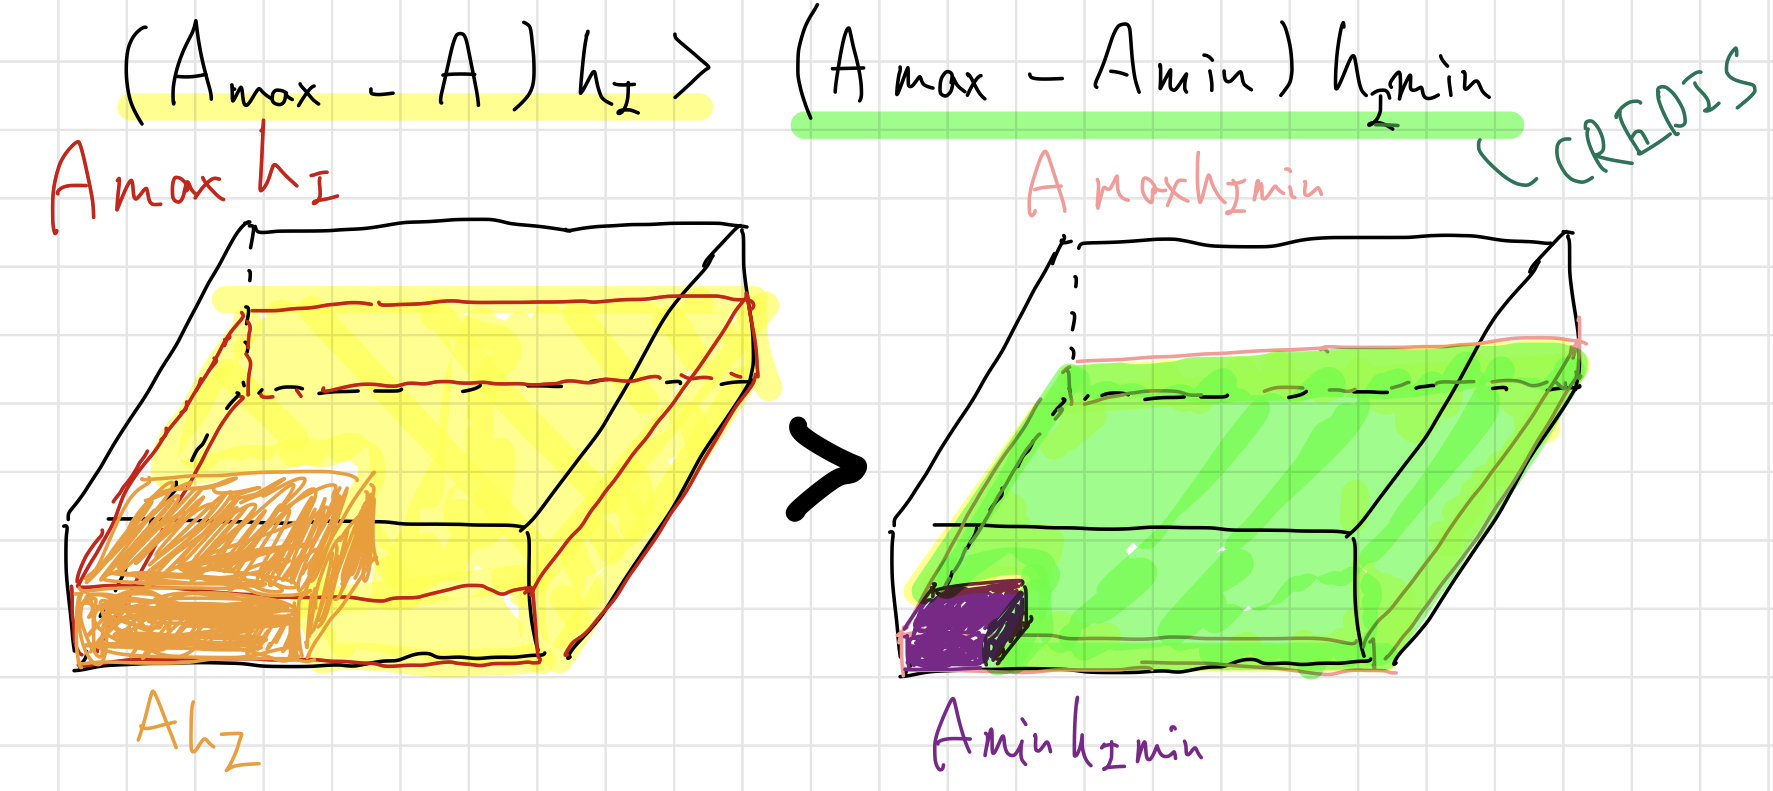
\includegraphics{lakeice_volume.jpeg}

\begin{eqnarray}
    h_I^{*** } = V^{free} + \frac{A_I^{n+1} h_I^{m+1}}{A_I^{max}}
\end{eqnarray}

The deficient water is come from the snow. The snow depth is now updated

\begin{eqnarray}
    h_S^{*** } = A_I^{n+1}\frac{h_S^{***}}{A_{max}-\frac{V_0^{free}}{h_I^{*** }}}
\end{eqnarray}

Finally, check if the snow is under water.

\begin{eqnarray}
    h_S^{n+1} = \mathrm{min}(h_S^{*** }, \frac{\rho_O-\rho_I}{\rho_S}h_I^{*** })
\end{eqnarray}

and the ice thickness is also updated.

\begin{eqnarray}
    h_I^{n+1} = h_I^{*** } + \frac{\rho_S}{\rho_I} (h_S^{*** }-h_S^{n+1})
\end{eqnarray}

The growth rate of the lake ice is

\begin{eqnarray}
    W_I^n = \frac{\rho_S A_I^{n+1}h_I^{n+1} - V_I'}{\rho_I \Delta t}
\end{eqnarray}

\begin{eqnarray}
    W_I^{n+1} = \frac{\rho_S A_I^{n+1}h_I^{n+1} - V_I^{n+1}}{\rho_I \Delta t}
\end{eqnarray}

The growth rate of the snow is

\begin{eqnarray}
    W_S^n =  \frac{\rho_S A_I^{n+1}h_S^{n+1} - V_S'}{\rho_S \Delta t}
\end{eqnarray}

\begin{eqnarray}
    W_S^{n+1} =  \frac{\rho_S A_I^{n+1}h_S^{n+1} - V_S^{n+1}}{\rho_S \Delta t}
\end{eqnarray}

The surface salinity flux \(F_S\) is

\begin{eqnarray}
    F_S = S_I(W_I-F_W^{SB}{''})
\end{eqnarray}

The freshwater flux \(F_W\) is

\begin{eqnarray}
    F_W(1) = - F_W + \frac{L_f}{C_p} \Big(W_I^{n+1}+W_S^{n+1}-Sn + \Delta F_W^{EV}\Big)
\end{eqnarray}

塩分変化に関係する分?

\begin{eqnarray}
    F_W(2) =F_W^{EV} - F_W^{PR} - R_{off} + W_S^n + W_I^n
\end{eqnarray}

\hypertarget{physical-formulation-processes-lakepo-20-written-in-jan-2021}{%
\subsection{\texorpdfstring{11.4 Physical formulation \& processes
\texttt{{[}LAKEPO{]}} {[}20\% Written in Jan,
2021{]}}{11.4 Physical formulation \& processes {[}LAKEPO{]} {[}20\% Written in Jan, 2021{]}}}\label{physical-formulation-processes-lakepo-20-written-in-jan-2021}}

\texttt{lakepo.F}

\hypertarget{set-parameters}{%
\subsubsection{Set parameters}\label{set-parameters}}

\hypertarget{diffusion-tracer-flux-vdiffl}{%
\paragraph{\texorpdfstring{Diffusion tracer flux
\texttt{{[}VDIFFL{]}}}{Diffusion tracer flux {[}VDIFFL{]}}}\label{diffusion-tracer-flux-vdiffl}}

\begin{itemize}
\tightlist
\item
  Inputs
\end{itemize}

Though several valuables are written, they are not used here.

\begin{itemize}
\tightlist
\item
  Outputs
\end{itemize}

\setlength\LTleft{0pt}\setlength\LTright{0pt}\begin{longtable}[]{@{}lllll@{}}
\toprule\relax
Meaning & Presentation & Variable & dimension & unit\tabularnewline
\midrule\relax
\endhead
vertical diffusion coefficient & \(K_V\) & AHV & IJLDIM, NLZDIM
&\tabularnewline
\bottomrule
\end{longtable}

\begin{itemize}
\tightlist
\item
  Parameters
\end{itemize}

\setlength\LTleft{0pt}\setlength\LTright{0pt}\begin{longtable}[]{@{}lllll@{}}
\toprule\relax
\begin{minipage}[b]{0.43\columnwidth}\raggedright
Meaning\strut
\end{minipage} & \begin{minipage}[b]{0.11\columnwidth}\raggedright
Presentation\strut
\end{minipage} & \begin{minipage}[b]{0.14\columnwidth}\raggedright
Variable\strut
\end{minipage} & \begin{minipage}[b]{0.05\columnwidth}\raggedright
unit\strut
\end{minipage} & \begin{minipage}[b]{0.12\columnwidth}\raggedright
value\strut
\end{minipage}\tabularnewline
\midrule\relax
\endhead
\begin{minipage}[t]{0.43\columnwidth}\raggedright
vertical diffusion coefficient at the surface layer\strut
\end{minipage} & \begin{minipage}[t]{0.11\columnwidth}\raggedright
\(K_{V0}\)\strut
\end{minipage} & \begin{minipage}[t]{0.14\columnwidth}\raggedright
AHVL0(NZ=KLMAX)\strut
\end{minipage} & \begin{minipage}[t]{0.05\columnwidth}\raggedright
\strut
\end{minipage} & \begin{minipage}[t]{0.12\columnwidth}\raggedright
\(k\times 1.0\)\strut
\end{minipage}\tabularnewline
\bottomrule
\end{longtable}

The case considered in COCO4 is that(
\href{https://ccsr.aori.u-tokyo.ac.jp/~hasumi/COCO/coco4.pdf}{Hasumi,
2015, Section 1.2}): 1. Diffusive flux of tracer follows the Fick's law.
2. Diffusuion coefficient tensor is diagonal, and its horizontal
component is identical.

Here, the vertical diffusion coefficent \(K_V\) is simply set as

\begin{eqnarray}
    K_V(k) = K_{V0} k
\end{eqnarray}

\hypertarget{estimate-the-advection-and-diffusion-terms-of-the-tracer-equations-flxtrcl}{%
\paragraph{\texorpdfstring{11.3.2 Estimate the advection and diffusion
terms of the tracer equations
\texttt{{[}FLXTRCL{]}}}{11.3.2 Estimate the advection and diffusion terms of the tracer equations {[}FLXTRCL{]}}}\label{estimate-the-advection-and-diffusion-terms-of-the-tracer-equations-flxtrcl}}

\begin{itemize}
\tightlist
\item
  Inputs
\end{itemize}

\setlength\LTleft{0pt}\setlength\LTright{0pt}\begin{longtable}[]{@{}lllll@{}}
\toprule\relax
Meaning & Presentation & Variable & dimension & unit\tabularnewline
\midrule\relax
\endhead
vertical diffusion coefficient & \(K_V\) & AHV & IJLDIM, NLZDIM
&\tabularnewline
water temperature & \(T\) & TX & IJLDIM, NLZDIM, NLTDIM &\tabularnewline
water depth & \(h\) & HX & IJLDIM &\tabularnewline
\bottomrule
\end{longtable}

\begin{itemize}
\tightlist
\item
  Outputs
\end{itemize}

\setlength\LTleft{0pt}\setlength\LTright{0pt}\begin{longtable}[]{@{}lllll@{}}
\toprule\relax
Meaning & Presentation & Variable & dimension & unit\tabularnewline
\midrule\relax
\endhead
vertical component of diffusive tracer flux & \(F_D\) & ADT & IJLDIM,
NLZDIM, NLTDIM &\tabularnewline
& \(\frac{F_D}{D(k-\frac{1}{2})}\) & DIFFZ & IJLDIM, NLZDIM
&\tabularnewline
\bottomrule
\end{longtable}

\begin{itemize}
\tightlist
\item
  Internal variables
\end{itemize}

\setlength\LTleft{0pt}\setlength\LTright{0pt}\begin{longtable}[]{@{}lllll@{}}
\toprule\relax
Meaning & Presentation & Variable & dimension & unit\tabularnewline
\midrule\relax
\endhead
& & TH & IJLDIM, NLZDIM, NLTDIM &\tabularnewline
& \(h'\) & HZBOT & IJLDIM &\tabularnewline
\bottomrule
\end{longtable}

-Parameters

\setlength\LTleft{0pt}\setlength\LTright{0pt}\begin{longtable}[]{@{}lllll@{}}
\toprule\relax
\begin{minipage}[b]{0.37\columnwidth}\raggedright
Meaning\strut
\end{minipage} & \begin{minipage}[b]{0.08\columnwidth}\raggedright
Presentation\strut
\end{minipage} & \begin{minipage}[b]{0.09\columnwidth}\raggedright
Variable\strut
\end{minipage} & \begin{minipage}[b]{0.09\columnwidth}\raggedright
unit\strut
\end{minipage} & \begin{minipage}[b]{0.22\columnwidth}\raggedright
value\strut
\end{minipage}\tabularnewline
\midrule\relax
\endhead
\begin{minipage}[t]{0.37\columnwidth}\raggedright
thickness of each lake level\strut
\end{minipage} & \begin{minipage}[t]{0.08\columnwidth}\raggedright
\(D\)\strut
\end{minipage} & \begin{minipage}[t]{0.09\columnwidth}\raggedright
DZ(NLZDIM)\strut
\end{minipage} & \begin{minipage}[t]{0.09\columnwidth}\raggedright
\(\mathrm{cm}\)\strut
\end{minipage} & \begin{minipage}[t]{0.22\columnwidth}\raggedright
\(0, S_0(1), S_0(2), S_0(3),S_0(4)\)\strut
\end{minipage}\tabularnewline
\begin{minipage}[t]{0.37\columnwidth}\raggedright
\strut
\end{minipage} & \begin{minipage}[t]{0.08\columnwidth}\raggedright
\(S\)\strut
\end{minipage} & \begin{minipage}[t]{0.09\columnwidth}\raggedright
DS(NLZDIM)\strut
\end{minipage} & \begin{minipage}[t]{0.09\columnwidth}\raggedright
\(\mathrm{ND}\)\strut
\end{minipage} & \begin{minipage}[t]{0.22\columnwidth}\raggedright
\strut
\end{minipage}\tabularnewline
\begin{minipage}[t]{0.37\columnwidth}\raggedright
thickness of the lake model's top level\strut
\end{minipage} & \begin{minipage}[t]{0.08\columnwidth}\raggedright
\(D_1\)\strut
\end{minipage} & \begin{minipage}[t]{0.09\columnwidth}\raggedright
DZ1\strut
\end{minipage} & \begin{minipage}[t]{0.09\columnwidth}\raggedright
\(\mathrm{cm}\)\strut
\end{minipage} & \begin{minipage}[t]{0.22\columnwidth}\raggedright
\(1.0\times 10^2\)\strut
\end{minipage}\tabularnewline
\begin{minipage}[t]{0.37\columnwidth}\raggedright
Ratio of the thickness of the each layer in sigma coordinate\strut
\end{minipage} & \begin{minipage}[t]{0.08\columnwidth}\raggedright
\(S_0\)\strut
\end{minipage} & \begin{minipage}[t]{0.09\columnwidth}\raggedright
DS0(NLZDIM-1)\strut
\end{minipage} & \begin{minipage}[t]{0.09\columnwidth}\raggedright
\(\mathrm{ND}\)\strut
\end{minipage} & \begin{minipage}[t]{0.22\columnwidth}\raggedright
\(0.1, 0.1, 0.2, 0.6\)\strut
\end{minipage}\tabularnewline
\bottomrule
\end{longtable}

Supposing that the thickness of the 1st top layer (\(k=2\)) is \(D_1\),

\begin{eqnarray}
    D(2) = D_1
\end{eqnarray}

the thickness of the remaining water column (\(h'\)) is presented by

\begin{eqnarray}
    h' = h - D_1
\end{eqnarray}

The thickness of each remaining layer (\(k=3,4,5,6\)) is

\begin{eqnarray}
    D(k) = S(k) {h'}
\end{eqnarray}

Then, the component of the diffusive tracer flux is represented by

\begin{eqnarray}
    F_D = K_V \frac{\partial T}{\partial z}
\end{eqnarray}

practically,

\begin{eqnarray}
    F_D(k) = K_V(k) \frac{T(k-1)-T(k)}{\frac{D(k-1)+D(k)}{2}} - K_V(k+1) \frac{T(k)-T(k+1)}{\frac{D(k)+D(k+1)}{2}}
\end{eqnarray}

\hypertarget{slvtrcl}{%
\paragraph{SLVTRCL}\label{slvtrcl}}

\begin{itemize}
\tightlist
\item
  Inputs
\end{itemize}

\setlength\LTleft{0pt}\setlength\LTright{0pt}\begin{longtable}[]{@{}lllll@{}}
\toprule\relax
Meaning & Presentation & Variable & dimension & unit\tabularnewline
\midrule\relax
\endhead
vertical component of diffusive tracer flux & \(F_D\) & ADT & IJLDIM,
NLZDIM, NLTDIM &\tabularnewline
& \(\frac{F_D}{D(k-\frac{1}{2})}\) & DIFFZ & IJLDIM, NLZDIM
&\tabularnewline
minimum depth of lake & & HXMIN & & \(\mathrm{cm}\)\tabularnewline
heat flux & & FT & & \(\mathrm{K cm/s}\)\tabularnewline
absorbed shortwave & & SWABS & &
\(\mathrm{erg/cm^2/sec}\)\tabularnewline
& & FS & &\tabularnewline
time step & \(\Delta t\) & TS & &\tabularnewline
surface-type fraction (lake) & \$\$ & LKFRAC & IJLDIM &
{[}-{]}\tabularnewline
\bottomrule
\end{longtable}

\begin{itemize}
\tightlist
\item
  Outputs
\end{itemize}

\setlength\LTleft{0pt}\setlength\LTright{0pt}\begin{longtable}[]{@{}lllll@{}}
\toprule\relax
Meaning & Presentation & Variable & dimension & unit\tabularnewline
\midrule\relax
\endhead
lake water deficient & & XHD & IJLDIM & \(\mathrm{cm}\)\tabularnewline
\bottomrule
\end{longtable}

\begin{eqnarray}
    A_A(k) = -\frac{K_V(k)}{\frac{D(k-1)+D(k)}{2}} \Delta t
\end{eqnarray}

\begin{eqnarray}
    A_C(k) = -\frac{K_V(k+1)}{\frac{D(k)+D(k+1)}{2}} \Delta t
\end{eqnarray}

\begin{eqnarray}
    A_B(k) = D)k-A_A(k)-A(k)
\end{eqnarray}

\begin{itemize}
\tightlist
\item
  THOMASL Solve the linear equations expressed by tri-diagonal matrix.
  (original files ./ocean/utrdg.F)
\end{itemize}

Then, \begin{eqnarray}
    T(k)=T(k)+ F_D(k)\Delta t
\end{eqnarray}

\begin{eqnarray}
    h_D = -F_T \Delta t
\end{eqnarray}

\begin{eqnarray}
    V_D = \mathrm{max}(h_{min}-h - h_D, 0) R_{lake}
\end{eqnarray}

\begin{eqnarray}
    h_D = \mathrm{max}(h_D,h_{min}-h)
\end{eqnarray}

Then, the deficient water is added.

\begin{eqnarray}
    h = h + h_D
\end{eqnarray}

\begin{eqnarray}
    h_{BOT}=h-D_1
\end{eqnarray}

ここで、

If \(h_D\ge0\), \(D^{top}=h_D S(\mathrm{KLEND})\) and \(D^{bottom}=0\)

If \(h_D\ge0\), 下からループ

\begin{eqnarray}
    T(k) = T(k) + \frac{  T(k-1) D^{top}}{h_{BOT}S(k)}
\end{eqnarray}

\begin{eqnarray}
    D
\end{eqnarray}

\hypertarget{ovturnl}{%
\paragraph{OVTURNL}\label{ovturnl}}

Reference:
\href{https://ccsr.aori.u-tokyo.ac.jp/~hasumi/COCO/coco4.pdf}{Hasumi,
2015, Section 4.1}

Let us consider finite difference discretization of a flux-form,
one-dimensional advection equation for tracer \(\psi\).

\begin{eqnarray}
    \frac{\partial \psi}{\partial t} + \frac{\partial}{\partial z} (w\psi) = 0
\end{eqnarray}

\begin{itemize}
\tightlist
\item
  Inputs
\end{itemize}

\setlength\LTleft{0pt}\setlength\LTright{0pt}\begin{longtable}[]{@{}lllll@{}}
\toprule\relax
Meaning & Presentation & Variable & dimension & unit\tabularnewline
\midrule\relax
\endhead
\(depth of water column\) & \(h\) & H & &\tabularnewline
time step & \(\Delta t\) & TS & &\tabularnewline
\bottomrule
\end{longtable}

\begin{itemize}
\tightlist
\item
  Outputs
\end{itemize}

\setlength\LTleft{0pt}\setlength\LTright{0pt}\begin{longtable}[]{@{}lllll@{}}
\toprule\relax
Meaning & Presentation & Variable & dimension & unit\tabularnewline
\midrule\relax
\endhead
& & R & &\tabularnewline
\bottomrule
\end{longtable}

The unit of XHD will be changed to \(\mathrm{kg/m2}\) after this module
(in \texttt{MATDRV}).

\hypertarget{setting-vertical-diffusion-and-viscosity-coefficients-vdiffl}{%
\subsubsection{\texorpdfstring{11.3.1 Setting vertical diffusion and
viscosity coefficients
\texttt{{[}VDIFFL{]}}}{11.3.1 Setting vertical diffusion and viscosity coefficients {[}VDIFFL{]}}}\label{setting-vertical-diffusion-and-viscosity-coefficients-vdiffl}}

Reference:
\href{https://ccsr.aori.u-tokyo.ac.jp/~hasumi/COCO/coco4.pdf}{Hasumi,
2015, Section 1}

\begin{itemize}
\tightlist
\item
  Variables
\end{itemize}

\setlength\LTleft{0pt}\setlength\LTright{0pt}\begin{longtable}[]{@{}lllll@{}}
\toprule\relax
\begin{minipage}[b]{0.44\columnwidth}\raggedright
Meaning\strut
\end{minipage} & \begin{minipage}[b]{0.15\columnwidth}\raggedright
Presentation\strut
\end{minipage} & \begin{minipage}[b]{0.07\columnwidth}\raggedright
Variable\strut
\end{minipage} & \begin{minipage}[b]{0.10\columnwidth}\raggedright
dimension\strut
\end{minipage} & \begin{minipage}[b]{0.10\columnwidth}\raggedright
unit\strut
\end{minipage}\tabularnewline
\midrule\relax
\endhead
\begin{minipage}[t]{0.44\columnwidth}\raggedright
the fraction of shortwave radiation absorved by the lake's z-level\strut
\end{minipage} & \begin{minipage}[t]{0.15\columnwidth}\raggedright
\strut
\end{minipage} & \begin{minipage}[t]{0.07\columnwidth}\raggedright
SWCONV\strut
\end{minipage} & \begin{minipage}[t]{0.10\columnwidth}\raggedright
IJLDIM, NLZDIM\strut
\end{minipage} & \begin{minipage}[t]{0.10\columnwidth}\raggedright
\(\mathrm{ND}\)\strut
\end{minipage}\tabularnewline
\begin{minipage}[t]{0.44\columnwidth}\raggedright
\strut
\end{minipage} & \begin{minipage}[t]{0.15\columnwidth}\raggedright
\strut
\end{minipage} & \begin{minipage}[t]{0.07\columnwidth}\raggedright
AA\strut
\end{minipage} & \begin{minipage}[t]{0.10\columnwidth}\raggedright
IJLDIM, NLZDIM\strut
\end{minipage} & \begin{minipage}[t]{0.10\columnwidth}\raggedright
\strut
\end{minipage}\tabularnewline
\begin{minipage}[t]{0.44\columnwidth}\raggedright
\strut
\end{minipage} & \begin{minipage}[t]{0.15\columnwidth}\raggedright
\strut
\end{minipage} & \begin{minipage}[t]{0.07\columnwidth}\raggedright
AB\strut
\end{minipage} & \begin{minipage}[t]{0.10\columnwidth}\raggedright
IJLDIM, NLZDIM\strut
\end{minipage} & \begin{minipage}[t]{0.10\columnwidth}\raggedright
\strut
\end{minipage}\tabularnewline
\begin{minipage}[t]{0.44\columnwidth}\raggedright
\strut
\end{minipage} & \begin{minipage}[t]{0.15\columnwidth}\raggedright
\strut
\end{minipage} & \begin{minipage}[t]{0.07\columnwidth}\raggedright
AC\strut
\end{minipage} & \begin{minipage}[t]{0.10\columnwidth}\raggedright
IJLDIM, NLZDIM\strut
\end{minipage} & \begin{minipage}[t]{0.10\columnwidth}\raggedright
\strut
\end{minipage}\tabularnewline
\begin{minipage}[t]{0.44\columnwidth}\raggedright
\strut
\end{minipage} & \begin{minipage}[t]{0.15\columnwidth}\raggedright
\strut
\end{minipage} & \begin{minipage}[t]{0.07\columnwidth}\raggedright
DH\strut
\end{minipage} & \begin{minipage}[t]{0.10\columnwidth}\raggedright
IJLDIM\strut
\end{minipage} & \begin{minipage}[t]{0.10\columnwidth}\raggedright
\strut
\end{minipage}\tabularnewline
\begin{minipage}[t]{0.44\columnwidth}\raggedright
thickness of the layers from the 2nd to the bottom\strut
\end{minipage} & \begin{minipage}[t]{0.15\columnwidth}\raggedright
\(h_B\)\strut
\end{minipage} & \begin{minipage}[t]{0.07\columnwidth}\raggedright
HZBOT\strut
\end{minipage} & \begin{minipage}[t]{0.10\columnwidth}\raggedright
IJLDIM\strut
\end{minipage} & \begin{minipage}[t]{0.10\columnwidth}\raggedright
\(\mathrm{cm}\)\strut
\end{minipage}\tabularnewline
\begin{minipage}[t]{0.44\columnwidth}\raggedright
\strut
\end{minipage} & \begin{minipage}[t]{0.15\columnwidth}\raggedright
\strut
\end{minipage} & \begin{minipage}[t]{0.07\columnwidth}\raggedright
HXBOT\strut
\end{minipage} & \begin{minipage}[t]{0.10\columnwidth}\raggedright
IJLDIM\strut
\end{minipage} & \begin{minipage}[t]{0.10\columnwidth}\raggedright
\strut
\end{minipage}\tabularnewline
\begin{minipage}[t]{0.44\columnwidth}\raggedright
\strut
\end{minipage} & \begin{minipage}[t]{0.15\columnwidth}\raggedright
\strut
\end{minipage} & \begin{minipage}[t]{0.07\columnwidth}\raggedright
DZB\strut
\end{minipage} & \begin{minipage}[t]{0.10\columnwidth}\raggedright
IJLDIM\strut
\end{minipage} & \begin{minipage}[t]{0.10\columnwidth}\raggedright
\strut
\end{minipage}\tabularnewline
\begin{minipage}[t]{0.44\columnwidth}\raggedright
\strut
\end{minipage} & \begin{minipage}[t]{0.15\columnwidth}\raggedright
\strut
\end{minipage} & \begin{minipage}[t]{0.07\columnwidth}\raggedright
DZT\strut
\end{minipage} & \begin{minipage}[t]{0.10\columnwidth}\raggedright
IJLDIM\strut
\end{minipage} & \begin{minipage}[t]{0.10\columnwidth}\raggedright
\strut
\end{minipage}\tabularnewline
\begin{minipage}[t]{0.44\columnwidth}\raggedright
\strut
\end{minipage} & \begin{minipage}[t]{0.15\columnwidth}\raggedright
\(I^{-\frac{1}{2}}(z)\)\strut
\end{minipage} & \begin{minipage}[t]{0.07\columnwidth}\raggedright
RADUP\strut
\end{minipage} & \begin{minipage}[t]{0.10\columnwidth}\raggedright
\strut
\end{minipage} & \begin{minipage}[t]{0.10\columnwidth}\raggedright
\(\mathrm{ND}\)\strut
\end{minipage}\tabularnewline
\begin{minipage}[t]{0.44\columnwidth}\raggedright
shortwave radiation flux at an arbitrary depth\strut
\end{minipage} & \begin{minipage}[t]{0.15\columnwidth}\raggedright
\(I^{+\frac{1}{2}}(z)\)\strut
\end{minipage} & \begin{minipage}[t]{0.07\columnwidth}\raggedright
RADDN\strut
\end{minipage} & \begin{minipage}[t]{0.10\columnwidth}\raggedright
\strut
\end{minipage} & \begin{minipage}[t]{0.10\columnwidth}\raggedright
\(\mathrm{ND}\)\strut
\end{minipage}\tabularnewline
\begin{minipage}[t]{0.44\columnwidth}\raggedright
Depth of each level\strut
\end{minipage} & \begin{minipage}[t]{0.15\columnwidth}\raggedright
\(D_H\)\strut
\end{minipage} & \begin{minipage}[t]{0.07\columnwidth}\raggedright
DEPTH\strut
\end{minipage} & \begin{minipage}[t]{0.10\columnwidth}\raggedright
\strut
\end{minipage} & \begin{minipage}[t]{0.10\columnwidth}\raggedright
\(\mathrm{cm}\)\strut
\end{minipage}\tabularnewline
\begin{minipage}[t]{0.44\columnwidth}\raggedright
the fraction of shortwave radiation absorved by the lake's z-level\strut
\end{minipage} & \begin{minipage}[t]{0.15\columnwidth}\raggedright
\(\Delta I(z)\)\strut
\end{minipage} & \begin{minipage}[t]{0.07\columnwidth}\raggedright
SWCNV1\strut
\end{minipage} & \begin{minipage}[t]{0.10\columnwidth}\raggedright
NLZDIM\strut
\end{minipage} & \begin{minipage}[t]{0.10\columnwidth}\raggedright
\(\mathrm{ND}\)\strut
\end{minipage}\tabularnewline
\begin{minipage}[t]{0.44\columnwidth}\raggedright
total of abrsorbed shortwave radiation\strut
\end{minipage} & \begin{minipage}[t]{0.15\columnwidth}\raggedright
\strut
\end{minipage} & \begin{minipage}[t]{0.07\columnwidth}\raggedright
TSWCNV\strut
\end{minipage} & \begin{minipage}[t]{0.10\columnwidth}\raggedright
IJLDIM\strut
\end{minipage} & \begin{minipage}[t]{0.10\columnwidth}\raggedright
\(\mathrm{ND}\)\strut
\end{minipage}\tabularnewline
\bottomrule
\end{longtable}

\begin{itemize}
\tightlist
\item
  parameters
\end{itemize}

\setlength\LTleft{0pt}\setlength\LTright{0pt}\begin{longtable}[]{@{}lllll@{}}
\toprule\relax
\begin{minipage}[b]{0.31\columnwidth}\raggedright
Meaning\strut
\end{minipage} & \begin{minipage}[b]{0.19\columnwidth}\raggedright
Presentation\strut
\end{minipage} & \begin{minipage}[b]{0.08\columnwidth}\raggedright
Variable\strut
\end{minipage} & \begin{minipage}[b]{0.12\columnwidth}\raggedright
unit\strut
\end{minipage} & \begin{minipage}[b]{0.17\columnwidth}\raggedright
value\strut
\end{minipage}\tabularnewline
\midrule\relax
\endhead
\begin{minipage}[t]{0.31\columnwidth}\raggedright
\strut
\end{minipage} & \begin{minipage}[t]{0.19\columnwidth}\raggedright
\(E_l\)\strut
\end{minipage} & \begin{minipage}[t]{0.08\columnwidth}\raggedright
emeltl\strut
\end{minipage} & \begin{minipage}[t]{0.12\columnwidth}\raggedright
\(\mathrm{J/kg}\)\strut
\end{minipage} & \begin{minipage}[t]{0.17\columnwidth}\raggedright
\(\mathrm{3.4\times 10^5}\)\strut
\end{minipage}\tabularnewline
\begin{minipage}[t]{0.31\columnwidth}\raggedright
density of sea water\strut
\end{minipage} & \begin{minipage}[t]{0.19\columnwidth}\raggedright
\(\rho_O\)\strut
\end{minipage} & \begin{minipage}[t]{0.08\columnwidth}\raggedright
rhoo\strut
\end{minipage} & \begin{minipage}[t]{0.12\columnwidth}\raggedright
\(\mathrm{g/cm^3}\)\strut
\end{minipage} & \begin{minipage}[t]{0.17\columnwidth}\raggedright
\(1.0\)\strut
\end{minipage}\tabularnewline
\begin{minipage}[t]{0.31\columnwidth}\raggedright
density of sea ice\strut
\end{minipage} & \begin{minipage}[t]{0.19\columnwidth}\raggedright
\(\rho_I\)\strut
\end{minipage} & \begin{minipage}[t]{0.08\columnwidth}\raggedright
rhoi\strut
\end{minipage} & \begin{minipage}[t]{0.12\columnwidth}\raggedright
\(\mathrm{g/cm^3}\)\strut
\end{minipage} & \begin{minipage}[t]{0.17\columnwidth}\raggedright
\(0.9\)\strut
\end{minipage}\tabularnewline
\begin{minipage}[t]{0.31\columnwidth}\raggedright
density of snow\strut
\end{minipage} & \begin{minipage}[t]{0.19\columnwidth}\raggedright
\(\rho_S\)\strut
\end{minipage} & \begin{minipage}[t]{0.08\columnwidth}\raggedright
rhos\strut
\end{minipage} & \begin{minipage}[t]{0.12\columnwidth}\raggedright
\(\mathrm{g/cm^3}\)\strut
\end{minipage} & \begin{minipage}[t]{0.17\columnwidth}\raggedright
\(0.33\)\strut
\end{minipage}\tabularnewline
\begin{minipage}[t]{0.31\columnwidth}\raggedright
latent heat fusion\strut
\end{minipage} & \begin{minipage}[t]{0.19\columnwidth}\raggedright
\(L_f\)\strut
\end{minipage} & \begin{minipage}[t]{0.08\columnwidth}\raggedright
hfus\strut
\end{minipage} & \begin{minipage}[t]{0.12\columnwidth}\raggedright
\(\mathrm{erg/g}\)\strut
\end{minipage} & \begin{minipage}[t]{0.17\columnwidth}\raggedright
\(E_l \times 1.0 \times 10^4\)\strut
\end{minipage}\tabularnewline
\begin{minipage}[t]{0.31\columnwidth}\raggedright
\strut
\end{minipage} & \begin{minipage}[t]{0.19\columnwidth}\raggedright
\(\frac{1}{\rho_O L_f}\)\strut
\end{minipage} & \begin{minipage}[t]{0.08\columnwidth}\raggedright
rrhfus\strut
\end{minipage} & \begin{minipage}[t]{0.12\columnwidth}\raggedright
\(\mathrm{cm^3/erg}\)\strut
\end{minipage} & \begin{minipage}[t]{0.17\columnwidth}\raggedright
\(1.0 /\rho_I/L_f\)\strut
\end{minipage}\tabularnewline
\begin{minipage}[t]{0.31\columnwidth}\raggedright
heat capacity of lake water\strut
\end{minipage} & \begin{minipage}[t]{0.19\columnwidth}\raggedright
\(C_{po}\)\strut
\end{minipage} & \begin{minipage}[t]{0.08\columnwidth}\raggedright
cpo\strut
\end{minipage} & \begin{minipage}[t]{0.12\columnwidth}\raggedright
\(\mathrm{erg/g/K}\)\strut
\end{minipage} & \begin{minipage}[t]{0.17\columnwidth}\raggedright
\(3.990\times 10^7\)\strut
\end{minipage}\tabularnewline
\begin{minipage}[t]{0.31\columnwidth}\raggedright
heat capacity of lake ice\strut
\end{minipage} & \begin{minipage}[t]{0.19\columnwidth}\raggedright
\(C_{pi}\)\strut
\end{minipage} & \begin{minipage}[t]{0.08\columnwidth}\raggedright
cpi\strut
\end{minipage} & \begin{minipage}[t]{0.12\columnwidth}\raggedright
\(\mathrm{erg/g/K}\)\strut
\end{minipage} & \begin{minipage}[t]{0.17\columnwidth}\raggedright
\(2.093\times 10^7\)\strut
\end{minipage}\tabularnewline
\begin{minipage}[t]{0.31\columnwidth}\raggedright
coeficient for a decreasing function of salinity\strut
\end{minipage} & \begin{minipage}[t]{0.19\columnwidth}\raggedright
\(\frac{\partial T}{\partial S}\)\strut
\end{minipage} & \begin{minipage}[t]{0.08\columnwidth}\raggedright
dtds\strut
\end{minipage} & \begin{minipage}[t]{0.12\columnwidth}\raggedright
\strut
\end{minipage} & \begin{minipage}[t]{0.17\columnwidth}\raggedright
\(-0.0543\)\strut
\end{minipage}\tabularnewline
\begin{minipage}[t]{0.31\columnwidth}\raggedright
\strut
\end{minipage} & \begin{minipage}[t]{0.19\columnwidth}\raggedright
\strut
\end{minipage} & \begin{minipage}[t]{0.08\columnwidth}\raggedright
dtdz\strut
\end{minipage} & \begin{minipage}[t]{0.12\columnwidth}\raggedright
\strut
\end{minipage} & \begin{minipage}[t]{0.17\columnwidth}\raggedright
\(-7.59\times 10^{-6}\)\strut
\end{minipage}\tabularnewline
\begin{minipage}[t]{0.31\columnwidth}\raggedright
fraction of the fast-attenuating portion\strut
\end{minipage} & \begin{minipage}[t]{0.19\columnwidth}\raggedright
\(R\)\strut
\end{minipage} & \begin{minipage}[t]{0.08\columnwidth}\raggedright
RRR\strut
\end{minipage} & \begin{minipage}[t]{0.12\columnwidth}\raggedright
\strut
\end{minipage} & \begin{minipage}[t]{0.17\columnwidth}\raggedright
\(5.0\times 10^{-1}\)\strut
\end{minipage}\tabularnewline
\begin{minipage}[t]{0.31\columnwidth}\raggedright
length scale for fast-attenuating portion\strut
\end{minipage} & \begin{minipage}[t]{0.19\columnwidth}\raggedright
\(\zeta_1\)\strut
\end{minipage} & \begin{minipage}[t]{0.08\columnwidth}\raggedright
ZETA1\strut
\end{minipage} & \begin{minipage}[t]{0.12\columnwidth}\raggedright
\strut
\end{minipage} & \begin{minipage}[t]{0.17\columnwidth}\raggedright
\(3.5\times 10^1\)\strut
\end{minipage}\tabularnewline
\begin{minipage}[t]{0.31\columnwidth}\raggedright
length scale for deeply penetrating spectral portion\strut
\end{minipage} & \begin{minipage}[t]{0.19\columnwidth}\raggedright
\(\zeta_2\)\strut
\end{minipage} & \begin{minipage}[t]{0.08\columnwidth}\raggedright
ZETA2\strut
\end{minipage} & \begin{minipage}[t]{0.12\columnwidth}\raggedright
\strut
\end{minipage} & \begin{minipage}[t]{0.17\columnwidth}\raggedright
\(2.3\times 10^3\)\strut
\end{minipage}\tabularnewline
\begin{minipage}[t]{0.31\columnwidth}\raggedright
thickness of the lake\strut
\end{minipage} & \begin{minipage}[t]{0.19\columnwidth}\raggedright
\(D(z)\)\strut
\end{minipage} & \begin{minipage}[t]{0.08\columnwidth}\raggedright
DZ(NZ=KLMAX)\strut
\end{minipage} & \begin{minipage}[t]{0.12\columnwidth}\raggedright
\(\mathrm{cm}\)\strut
\end{minipage} & \begin{minipage}[t]{0.17\columnwidth}\raggedright
\texttt{DZ1}\strut
\end{minipage}\tabularnewline
\begin{minipage}[t]{0.31\columnwidth}\raggedright
\strut
\end{minipage} & \begin{minipage}[t]{0.19\columnwidth}\raggedright
\(S(z)\)\strut
\end{minipage} & \begin{minipage}[t]{0.08\columnwidth}\raggedright
DS(NZ=KLMAX)\strut
\end{minipage} & \begin{minipage}[t]{0.12\columnwidth}\raggedright
\(\mathrm{ND}\)\strut
\end{minipage} & \begin{minipage}[t]{0.17\columnwidth}\raggedright
\texttt{DS0(K-KLSTR)}\strut
\end{minipage}\tabularnewline
\begin{minipage}[t]{0.31\columnwidth}\raggedright
thickness of the lake model's top level\strut
\end{minipage} & \begin{minipage}[t]{0.19\columnwidth}\raggedright
\$D(1) \$\strut
\end{minipage} & \begin{minipage}[t]{0.08\columnwidth}\raggedright
DZ1\strut
\end{minipage} & \begin{minipage}[t]{0.12\columnwidth}\raggedright
\(\mathrm{cm}\)\strut
\end{minipage} & \begin{minipage}[t]{0.17\columnwidth}\raggedright
\(1.0\times 10^2\)\strut
\end{minipage}\tabularnewline
\begin{minipage}[t]{0.31\columnwidth}\raggedright
\strut
\end{minipage} & \begin{minipage}[t]{0.19\columnwidth}\raggedright
\(S_0(z)\)\strut
\end{minipage} & \begin{minipage}[t]{0.08\columnwidth}\raggedright
DS0(NZ-1)\strut
\end{minipage} & \begin{minipage}[t]{0.12\columnwidth}\raggedright
\(\mathrm{ND}\)\strut
\end{minipage} & \begin{minipage}[t]{0.17\columnwidth}\raggedright
\(0.1, 0.1, 0.2, 0.6\)\strut
\end{minipage}\tabularnewline
\bottomrule
\end{longtable}

\begin{itemize}
\tightlist
\item
  \(\mathrm{erg}=10^{-7} \mathrm{J}\)
\end{itemize}

Reference:
\href{https://ccsr.aori.u-tokyo.ac.jp/~hasumi/COCO/coco4.pdf}{Hasumi,
2015, Section 3.2.4}

Then, the depth of each level is presented by

\begin{eqnarray}
    H(k) = \sum _{k=2} ^{k-1} H +D(k)
\end{eqnarray}

While incoming downward longwave radiation is completely absorbed within
a very thin surface layer, shortwave radiation can penetrate
significantly into depths. In order to take account of its effect,
shortwave radiation flux at an arbitary depth in the ocean is
parameterized by

\begin{eqnarray}
     I^{+\frac{1}{2}}(z)  = R e^{-\frac{D(z)}{\zeta_1}} + (1- R)e^{-\frac{D(z)}{\zeta_2}}
\end{eqnarray}

\begin{eqnarray}
    \Delta I(z) = I^{-\frac{1}{2}}(z) - I^{+\frac{1}{2}}(z)
\end{eqnarray}

where \(I(0)=1.0\). Here, shortwave radiation is split into two
portions: one is a fast-attenuating spectral portion and the other is a
deeply penetrating spectral portion, and these two portions attenuate
with length scales of \(\zeta_1\) and \(\zeta_2\), respectively.
\(\Delta I(z=2)\) is handed to the lake ice scheme (hence
\(\Delta I(z=2)\) is set to zero).

The residual is absorbed by the bottom layer.

\begin{eqnarray}
    \Delta I(z_{max}+1) = 1- \Sigma _{z=2}^{z_{max}}
\end{eqnarray}

For the preparation of the next step, the unit of \(\Delta I(z)\) is
modified. The new variable is represented as \(\Delta I_{tmp}(z)\) here.

\begin{eqnarray}
    \Delta I_{tmp}(z) = \frac{\Delta I(z)}{\rho_O {C_p}_o}
\end{eqnarray}

\hypertarget{thomasl}{%
\subsubsection{THOMASL}\label{thomasl}}

\hypertarget{convective-adjustment-for-the-unstable-water-column-ovtsetl}{%
\subsubsection{\texorpdfstring{11.3.4 Convective adjustment for the
unstable water column
\texttt{{[}OVTSETL{]}}}{11.3.4 Convective adjustment for the unstable water column {[}OVTSETL{]}}}\label{convective-adjustment-for-the-unstable-water-column-ovtsetl}}

Reference:
\href{https://ccsr.aori.u-tokyo.ac.jp/~hasumi/COCO/coco4.pdf}{Hasumi,
2015, Section 4.4}
